%\PassOptionsToPackage{usenames,dvipsnames}{xcolor}
\documentclass[compress,10pt,usenames,dvipsnames]{Presentation} % Add notesonly option to print the notes in each frame
%%%%%%%%%%%%%%%%%%%%%%%%%%%%%%%%%%%%%%%%%%%%%%%%%%

%
% Some useful commands
%
\begin{comment}
  \frame
      {
        \frametitle{List displayed step by step}
        text
      }
      
      frame environment commands
      command<#>{applies the command only on certain slides}
      ex:
      \textbf{Thislineisboldonallthreeslides.}
      \textbf<2>{Thislineisboldsolelyonthesecondslide.}
      \textbf<3>{Thislineisboldsolelyonthethirdslide.}
      
      \only<#>{text shown only on the specified slide}
      
      \uncover<slides>{text that occupies space,but is not shown except on the specified slides}
      
      \invisible<slides>{text is invisibale on the specified slides}
      
      \alt<slides>{<main text shown on specified slide>}{otherwise the alternative text is shown}
      
      \temporal<slides>{before specified slide}{on specified slide}{after specified slide}
      
      #-#
      
      #- all slides after #
      
      -#=1-#
      
      Highlighted environments
      \begin{beamerboxesrounded}{title}
      \end{beamerboxesrounded}
\end{comment}
%%%%%%%%%%%%%%%%%%%%%%%%%%%%%%%%%%%%%%%%%%%%%%%%%%
\begin{comment}
%Only one section and subsection shown at a time
\setbeamertemplate{headline}
{%
  \leavevmode%
  \begin{beamercolorbox}[wd=.5\paperwidth,ht=2.5ex,dp=2.125ex]{section in head/foot}% original dp=1.125ex
    \hbox to .5\paperwidth{\hfil\insertsectionhead\hfil}
  \end{beamercolorbox}%
  \begin{beamercolorbox}[wd=.5\paperwidth,ht=2.5ex,dp=2.125ex]{subsection in head/foot}%
    \hbox to .5\paperwidth{\hfil\insertsubsectionhead\hfil}
  \end{beamercolorbox}%
}
\newcommand{\tikzmark}[1]{\tikz[overlay,remember picture] \node (#1) {};}
\end{comment}
%%%%%%%%%%%%%%%%%%%%%%%%%%%%%%%%%%%%%%%%%%%%%%%%%%

\title[HATS\@LPC]{HATS@LPC} %\title[short title]{title}
\subtitle[JEC]{Jet Energy Corrections in CMS} %\subtitle[short subtitle]{subtitle}
\author[A. Perloff]{Alexx Perloff\inst{1} \& Ben Kreis\inst{2}} % \author[A. Perloff]{Alexx Perloff}
\institute[TAMU]
{
\begin{center}
  \inst{1}%
  Department of Physics and Astronomy\\
  Texas A{\&}M University\\
  %College Station, Texas 77843\\[1ex]
  %\texttt{aperloff@physics.tamu.edu}
  %\and
  \inst{2}%
  Fermilab\\
  %College Station, Texas 77843\\[1ex]
  %\texttt{aperloff@physics.tamu.edu}
  %\and
  \end{center}
}
\newdate{date}{30}{06}{2016}
\usdate
\date{\dayofweekname{30}{06}{2016}, \displaydate{date}}
%\date{\displaydate{date}}
%\date{\today}

%%%%%%%%%%%%%%%%%%%%%%%%%%%%%%%%%%%%%%%%%%%%%%%%%%
\begin{document}

\newlength{\residualSpace}

\frame {
  \begin{center}
    
\includegraphics[width=0.45in]{images/TAMULogoMaroonBox.jpg}\hspace{0.97in}
\includegraphics[width=2.0in]{images/FNAL-Logo-NAL-Blue.pdf}\hspace{0.97in}
\includegraphics[width=0.45in]{images/CMS_exp.png}
  \end{center}
  \vspace{-0.5cm}
  \titlepage
}

\section{Introduction}
\label{sec:introduction}
%!TEX root = ../2015_06_16-HATS-LPC-JEC.tex

\subsection{Why?}
\frame{
	\frametitle{Introduction to Jet Energy Corrections in CMS}
	\vspace*{-0.24cm}
	\begin{columns}
		\begin{column}{0.49\textwidth}
			\begin{block}{Why do we need jet energy corrections?}
					\begin{itemize}
						\item For an abundance of reasons, the CMS detector does not perfectly measure the $p_{T}$ of most of the jets
						\item Therefore it is not straightforward to translate the measured jet energy to the true particle or parton energy
						\item Reasons:
						\begin{itemize}
							\item Pileup can add extra energy to the jets making their response ($p_{T}^{measured}/p_{T}^{actual}$) too high
							\item The calorimeter response to particles is not constant in either $p_{T}^{RECO}$ or $\eta$
							\item The detector response varies with jet flavor and parton flavor
							\item etc.
						\end{itemize}
					\end{itemize}
				\end{block}
		\end{column}
		\begin{column}{0.49\textwidth}
			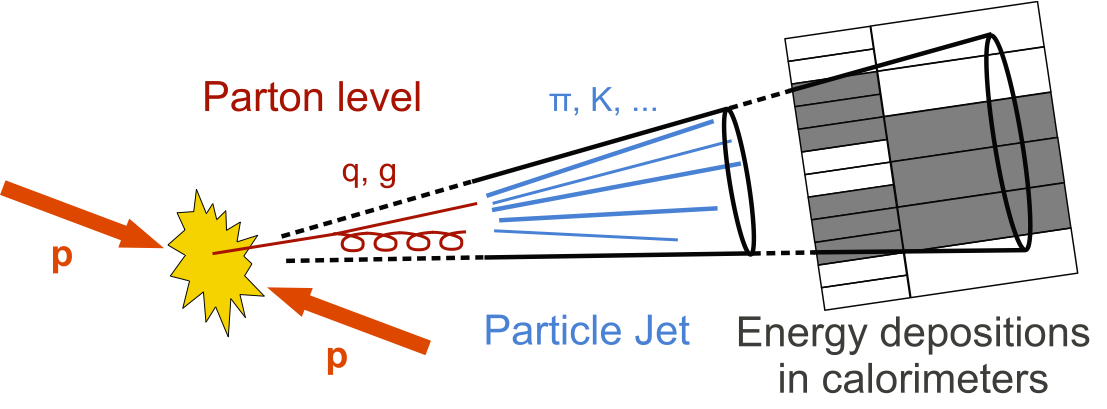
\includegraphics[width=\textwidth]{images/jetsatcmsand.png}\\
			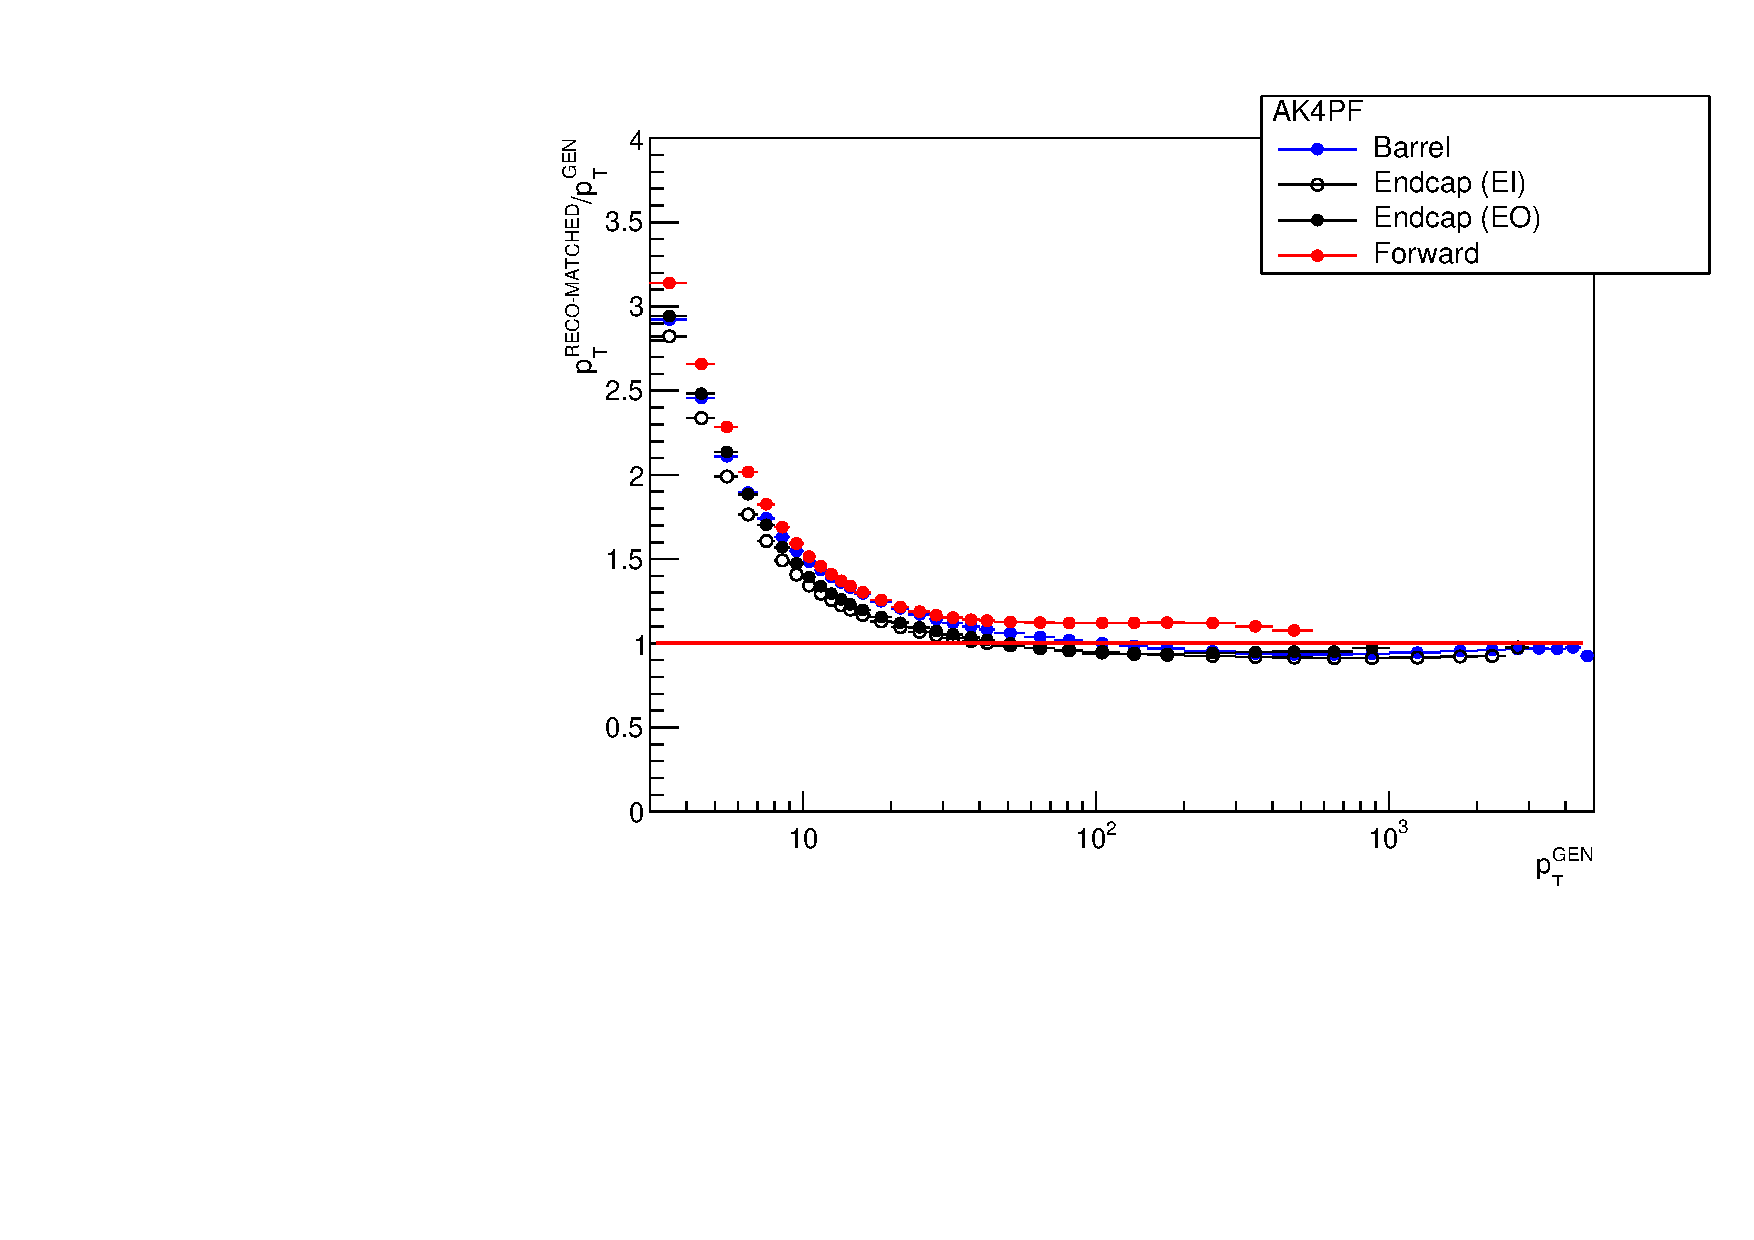
\includegraphics[width=\textwidth]{images/response.pdf}
		\end{column}
	\end{columns}
}

%---------------------------------------------------------------------------------------------------------------------------------------
\subsection{What?}
\frame{
	\frametitle{What are the JECs?}
	\vspace*{-0.24cm}
	\begin{block}{Definition}
		\begin{itemize}
			\item The jet energy corrections (JEC) are a set of functions, constants, and tools that allows the proper mapping of the measured jet energy to the energy of the initiating parton
		\end{itemize}
	\end{block}
	\vspace*{-0.15cm}
	\begin{block}{Factorized Approach}
		\begin{itemize}
			\item CMS has adopted a factorized solution to the problem of jet energy corrections, where each level of correction takes care of a different effect
			\begin{itemize}
				\item Each level of correction is essentially the application of a scale factor (correction) to the jet four momentum
				\item This scale factor depends on various event and jet related quantities ($\rho$, $p_{T}, \eta$, flavor, etc.)
				\item The levels of correction are applied sequentially (the output of each step is the input to the next) and with fixed order
			\end{itemize}
		\end{itemize}
	\end{block}
	\vspace*{-0.15cm}
	\begin{center}
		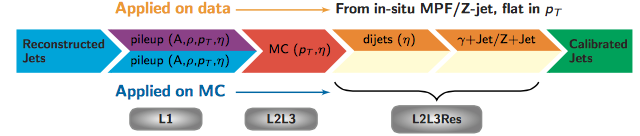
\includegraphics[width=10cm]{images/jecs.png}
	\end{center}
}
%---------------------------------------------------------------------------------------------------------------------------------------
\frame{
	\frametitle{JECs: A Factorized Approach}
	\begin{textblock}{12.3}(0.0,0.75)
		\begin{figure}
			 \scalebox{.9}{
				\documentclass[dvipsnames]{standalone}
\usepackage{color}
\usepackage{tikz}
\usetikzlibrary{arrows,shapes,shapes.multipart,backgrounds,calc,decorations.text,decorations.pathreplacing,matrix,shadings}
\tikzstyle{every picture}+=[remember picture]
\tikzstyle{na} = [baseline=-.5ex]

\begin{document}

\tikzstyle{levels} = [rectangle, draw, text width=6em, text centered, rounded corners, minimum height=2em, midway, shading=radial,outer color=Gray,middle color=white,inner color=white, Gray]
\tikzstyle{arrow} = [draw, -latex']
\tikzstyle{line} = [draw, -]

\newcommand*{\mytextstyle}{\sffamily\Large\bfseries\color{black!85}}
\newcommand{\myarrowstart}[9]{%
% inner radius, middle radius, outer radius, start angle,
% end angle, tip protusion angle, options, text
  \pgfmathsetmacro{\start}{#1}
  \pgfmathsetmacro{\rin}{#2}
  \pgfmathsetmacro{\rmid}{#3}
  \pgfmathsetmacro{\rout}{#4}
  \pgfmathsetmacro{\astart}{#5}
  \pgfmathsetmacro{\aend}{#6}
  \pgfmathsetmacro{\atip}{#7}
  \fill[#8] (\start+\astart,\rin) -- (\start+\aend,\rin) -- (\start+\aend+\atip,\rmid)
        -- (\start+\aend,\rout) -- (\start+\astart,\rout) -- (\start+\astart,\rmid)
        -- cycle;
  \node[font = \sffamily, align=center,text width=\aend-\astart,anchor = west, yshift=-0.0ex] (arrowend) at (\start+\astart,\rmid) {\mytextstyle{#9}};
%  \path[font = \sffamily, decoration = {text along path, text = {|\mytextstyle|#9},
%    text align = {align = center}, raise = -0.5ex}, decorate]
%    (\start+\astart+0.4*\atip,\rmid) -- (\start+\aend+0.4*\atip,\rmid);
}
\newcommand{\myarrow}[9]{%
% inner radius, middle radius, outer radius, start angle,
% end angle, tip protusion angle, options, text
  \pgfmathsetmacro{\start}{#1}
  \pgfmathsetmacro{\rin}{#2}
  \pgfmathsetmacro{\rmid}{#3}
  \pgfmathsetmacro{\rout}{#4}
  \pgfmathsetmacro{\astart}{#5}
  \pgfmathsetmacro{\aend}{#6}
  \pgfmathsetmacro{\atip}{#7}
  \fill[#8] (\start+\astart,\rin) -- (\start+\aend,\rin) -- (\start+\aend+\atip,\rmid) 
        -- (\start+\aend,\rout) -- (\start+\astart,\rout) -- (\start+\astart+\atip,\rmid)
        -- cycle;
  \path[font = \sffamily, decoration = {text along path, text = {|\mytextstyle|#9},
    text align = {align = center}, raise = -0.5ex}, decorate]
    (\start+\astart+0.75*\atip,\rmid) -- (\start+\aend+0.75*\atip,\rmid);
}
\newcommand{\myuphalfarrow}[9]{%
% inner radius, middle radius, outer radius, start angle,
% end angle, tip protusion angle, options, text
  \pgfmathsetmacro{\start}{#1}
  \pgfmathsetmacro{\rin}{#2}
  \pgfmathsetmacro{\rmid}{#3}
  \pgfmathsetmacro{\rout}{#4}
  \pgfmathsetmacro{\astart}{#5}
  \pgfmathsetmacro{\aend}{#6}
  \pgfmathsetmacro{\atip}{#7}
  \fill[#8] (\start+\astart,\rout) -- (\start+\aend,\rout) -- (\start+\aend+\atip,\rin) 
        -- (\start+\astart+\atip,\rin) -- cycle;
  \path[font = \sffamily, decoration = {text along path, text = {|\mytextstyle|#9},
    text align = {align = center}, raise = -0.5ex}, decorate]
    (\start+\astart+0.4*\atip,\rmid) -- (\start+\aend+0.4*\atip,\rmid);
}
\newcommand{\mylowhalfarrow}[9]{%
% inner radius, middle radius, outer radius, start angle,
% end angle, tip protusion angle, options, text
  \pgfmathsetmacro{\start}{#1}
  \pgfmathsetmacro{\rin}{#2}
  \pgfmathsetmacro{\rmid}{#3}
  \pgfmathsetmacro{\rout}{#4}
  \pgfmathsetmacro{\astart}{#5}
  \pgfmathsetmacro{\aend}{#6}
  \pgfmathsetmacro{\atip}{#7}
  \fill[#8] (\start+\astart+\atip,\rin) -- (\start+\aend+\atip,\rin) -- (\start+\aend,\rout)
        -- (\start+\astart,\rout) -- cycle;
  \path[font = \sffamily, decoration = {text along path, text = {|\mytextstyle|#9},
    text align = {align = center}, raise = -0.5ex}, decorate]
    (\start+\astart+0.4*\atip,\rmid) -- (\start+\aend+0.4*\atip,\rmid);
}
\newcommand{\myarrowend}[9]{%
% inner radius, middle radius, outer radius, start angle,
% end angle, tip protusion angle, options, text
  \pgfmathsetmacro{\start}{#1}
  \pgfmathsetmacro{\rin}{#2}
  \pgfmathsetmacro{\rmid}{#3}
  \pgfmathsetmacro{\rout}{#4}
  \pgfmathsetmacro{\astart}{#5}
  \pgfmathsetmacro{\aend}{#6}
  \pgfmathsetmacro{\atip}{#7}
  \fill[#8] (\start+\astart,\rin) -- (\start+\aend,\rin) -- (\start+\aend,\rmid)
        -- (\start+\aend,\rout) -- (\start+\astart,\rout) -- (\start+\astart+\atip,\rmid)
        -- cycle;
  \node[font = \sffamily, align=center,text width=\aend-\astart,anchor = west, yshift=-0.0ex] (arrowend) at (\start+\astart+0.75*\atip,\rmid) {\mytextstyle{#9}};
}

\begin{tikzpicture}[node distance = 2cm, auto, scale=0.8]
\scriptsize
    % Place nodes
    \myarrowstart{0}{0.5}{1.5}{2.5}{0}{1.75}{0.5}{Cyan,draw = Cyan, very thick}{\scriptsize{Reconstructed Jets}}

    \myuphalfarrow{1.95}{1.52}{1.75}{2.5}{0}{2.0}{0.5}{Purple,draw = Purple, very thick}{|\scriptsize|{MC + RC}}
    \mylowhalfarrow{1.95}{1.48}{1.}{0.5}{0}{2.0}{0.5}{Cyan,draw = Cyan, very thick}{|\scriptsize|{MC}}

    \node [font = \sffamily, align=left,text width=2.cm,anchor = west, yshift=-0.0ex] (l1data) at (2.4,2.2) {\mytextstyle\small\color{Black}\scriptsize{Pileup}};


    \myarrow{4.15}{0.5}{1.5}{2.5}{0}{2.95}{0.5}{Red!80,draw = Red!80, very thick}{|\scriptsize|{MC}}
    \node [font = \sffamily, align=left,text width=2.cm,anchor = west, yshift=-0.0ex] (l2l3) at (4.35,2.2) {\mytextstyle\small\color{Black}\scriptsize{Response $(p_{T},\eta)$ }};


    \myuphalfarrow{7.3}{1.52}{1.75}{2.5}{0}{1.9}{0.5}{BurntOrange,draw = BurntOrange, very thick}{|\scriptsize|{dijets}}
    \node [font = \sffamily, align=left,text width=2.cm,anchor = west, yshift=-0.0ex] (l2res) at (7.4,2.2) {\mytextstyle\small\color{Black}\scriptsize{Residuals$(\eta)$}};
    \mylowhalfarrow{7.3}{1.48}{1.25}{0.5}{0}{1.9}{0.5}{yellow!20,draw = yellow!20, very thick}{}


   \myuphalfarrow{9.4}{1.52}{1.75}{2.5}{0}{2.4}{0.5}{BurntOrange,draw = BurntOrange, very thick}{|\scriptsize|{   $\gamma$/Z$+$jet, MJB}}
    \node [font = \sffamily, align=left,text width=2.cm,anchor = west, yshift=-0.0ex] (l3res) at (9.6,2.2) {\mytextstyle\small\color{Black}\scriptsize{Residuals$(p_T)$}};
    \mylowhalfarrow{9.4}{1.48}{1.25}{0.5}{0}{2.4}{0.5}{yellow!20,draw = yellow!20, very thick}{}

 
   \myarrow{12.0}{0.5}{1.5}{2.5}{0}{1.}{0.5}{Yellow!80,draw = Yellow!80, very thick}{|\scriptsize|{MC}}
    \node [font = \sffamily, align=left,text width=2.cm,anchor = west, yshift=-0.0ex] (l5) at (12.,2.2) {\mytextstyle\small\color{Black}\scriptsize{ Flavor}};


    \myarrowend{13.20}{0.5}{1.5}{2.5}{0}{2.}{0.5}{Green!90,draw = Green!90, very thick}{\scriptsize{Calibrated Jets}}
    
    \node [font = \sffamily, align=left,text width=2.75cm,anchor = west, yshift=-0.0ex] (MC) at (2.25,0.) {\mytextstyle\small\color{RoyalBlue}Applied on MC};
    \node [font = \sffamily, align=left,text width=2.75cm,anchor = west, yshift=-0.0ex] (DATA) at (2.25,3.) {\mytextstyle\small\color{YellowOrange}Applied on data};

    \node [font = \sffamily, align=left,text width=5cm,anchor = west, yshift=-0.0ex] (INSITU) at (7.6,3.) %%{\mytextstyle\footnotesize{From in-situ MPF/Z-jet, flat in $p_{T}$}};
   {\mytextstyle\footnotesize{}};
    \node [font = \sffamily, align=left,text width=5cm,anchor = west, yshift=-0.0ex] (STARTBRACE) at (7.6,0.) {};
    \node [font = \sffamily, align=left,text width=5cm,anchor = west, yshift=-0.0ex] (ENDBRACE) at (12.65,0.5) {};
    \path[arrow,YellowOrange,thick, shorten <= -0.5cm] (DATA) -- (INSITU);
%    \draw [thick, decorate, decoration = {brace, amplitude = 10pt, mirror}, xshift = 0pt, yshift = 0pt] (7.25,0.75) -- (12.0,0.75) node [black, midway, xshift = 0cm, yshift = -0.8cm] {\mytextstyle\small{stuff}};
 %   \draw [thick, decorate, decoration = {brace, amplitude = 10pt, mirror}, xshift = 0pt, yshift = 0pt] (7.7,0.75) -- (12.65,0.75) node [levels, xshift = 0cm, yshift = -1.0cm] {\mytextstyle\scriptsize{L2L3Res}};

   \path[arrow,RoyalBlue,thick, shorten <= -0.5cm] (MC) -- (STARTBRACE);

 %   \node [levels, below of=MC, xshift = 3.6cm, yshift = 1.85cm, thick] (L1) {\mytextstyle\small{L1}};
 %   \node [levels, right of=L1, xshift = 4.4cm, yshift = -0.15cm, thick] (L2L3) {\mytextstyle\small{L2L3}};
\end{tikzpicture}

\end{document}

			}
			\label{fig:factorized_approach}
		\end{figure}
	\end{textblock}
	\vspace*{2.4cm}
	\begin{block}{Pileup (PU) Corrections}
		\begin{itemize}
			\footnotesize
			\item Pileup is the additional energy in a jet coming from all interactions \textbf{except} the primary vertex (PV) and it's underlying event (UE)
			\item The goal of the pileup (\textbf{L1}) corrections is to remove the energy inside a jet coming from pile-up events
			\begin{itemize}
				\footnotesize
				\item L1Offset - No longer used
				\item L1FastJet - The current standard
				\item Charged Hardron Subtraction - Remove the charged hadrons inside a jet which have a track coming from a pileup vertex
				\item Pileup Per Particle Identification (PUPPI) - the new kid on the block (more in section~\ref{})
			\end{itemize}
			\item Done on an {\color{blue}event-by-event} basis ($\rho$, $\mu$) and a {\color{red}jet-by-jet} basis ($p_{T}$, $\eta$, jet area)
			\item The first step in calculating these is MC based, but the corrections for data are scaled with L1Residual corrections
		\end{itemize}
	\end{block}
}
%---------------------------------------------------------------------------------------------------------------------------------------
\frame{
	\frametitle{JECs: A Factorized Approach}
	\begin{textblock}{12.3}(0.0,0.75)
		\begin{figure}
			 \scalebox{.9}{
				\documentclass[dvipsnames]{standalone}
\usepackage{color}
\usepackage{tikz}
\usetikzlibrary{arrows,shapes,shapes.multipart,backgrounds,calc,decorations.text,decorations.pathreplacing,matrix,shadings}
\tikzstyle{every picture}+=[remember picture]
\tikzstyle{na} = [baseline=-.5ex]

\begin{document}

\tikzstyle{levels} = [rectangle, draw, text width=6em, text centered, rounded corners, minimum height=2em, midway, shading=radial,outer color=Gray,middle color=white,inner color=white, Gray]
\tikzstyle{arrow} = [draw, -latex']
\tikzstyle{line} = [draw, -]

\newcommand*{\mytextstyle}{\sffamily\Large\bfseries\color{black!85}}
\newcommand{\myarrowstart}[9]{%
% inner radius, middle radius, outer radius, start angle,
% end angle, tip protusion angle, options, text
  \pgfmathsetmacro{\start}{#1}
  \pgfmathsetmacro{\rin}{#2}
  \pgfmathsetmacro{\rmid}{#3}
  \pgfmathsetmacro{\rout}{#4}
  \pgfmathsetmacro{\astart}{#5}
  \pgfmathsetmacro{\aend}{#6}
  \pgfmathsetmacro{\atip}{#7}
  \fill[#8] (\start+\astart,\rin) -- (\start+\aend,\rin) -- (\start+\aend+\atip,\rmid)
        -- (\start+\aend,\rout) -- (\start+\astart,\rout) -- (\start+\astart,\rmid)
        -- cycle;
  \node[font = \sffamily, align=center,text width=\aend-\astart,anchor = west, yshift=-0.0ex] (arrowend) at (\start+\astart,\rmid) {\mytextstyle{#9}};
%  \path[font = \sffamily, decoration = {text along path, text = {|\mytextstyle|#9},
%    text align = {align = center}, raise = -0.5ex}, decorate]
%    (\start+\astart+0.4*\atip,\rmid) -- (\start+\aend+0.4*\atip,\rmid);
}
\newcommand{\myarrow}[9]{%
% inner radius, middle radius, outer radius, start angle,
% end angle, tip protusion angle, options, text
  \pgfmathsetmacro{\start}{#1}
  \pgfmathsetmacro{\rin}{#2}
  \pgfmathsetmacro{\rmid}{#3}
  \pgfmathsetmacro{\rout}{#4}
  \pgfmathsetmacro{\astart}{#5}
  \pgfmathsetmacro{\aend}{#6}
  \pgfmathsetmacro{\atip}{#7}
  \fill[#8] (\start+\astart,\rin) -- (\start+\aend,\rin) -- (\start+\aend+\atip,\rmid) 
        -- (\start+\aend,\rout) -- (\start+\astart,\rout) -- (\start+\astart+\atip,\rmid)
        -- cycle;
  \path[font = \sffamily, decoration = {text along path, text = {|\mytextstyle|#9},
    text align = {align = center}, raise = -0.5ex}, decorate]
    (\start+\astart+0.75*\atip,\rmid) -- (\start+\aend+0.75*\atip,\rmid);
}
\newcommand{\myuphalfarrow}[9]{%
% inner radius, middle radius, outer radius, start angle,
% end angle, tip protusion angle, options, text
  \pgfmathsetmacro{\start}{#1}
  \pgfmathsetmacro{\rin}{#2}
  \pgfmathsetmacro{\rmid}{#3}
  \pgfmathsetmacro{\rout}{#4}
  \pgfmathsetmacro{\astart}{#5}
  \pgfmathsetmacro{\aend}{#6}
  \pgfmathsetmacro{\atip}{#7}
  \fill[#8] (\start+\astart,\rout) -- (\start+\aend,\rout) -- (\start+\aend+\atip,\rin) 
        -- (\start+\astart+\atip,\rin) -- cycle;
  \path[font = \sffamily, decoration = {text along path, text = {|\mytextstyle|#9},
    text align = {align = center}, raise = -0.5ex}, decorate]
    (\start+\astart+0.4*\atip,\rmid) -- (\start+\aend+0.4*\atip,\rmid);
}
\newcommand{\mylowhalfarrow}[9]{%
% inner radius, middle radius, outer radius, start angle,
% end angle, tip protusion angle, options, text
  \pgfmathsetmacro{\start}{#1}
  \pgfmathsetmacro{\rin}{#2}
  \pgfmathsetmacro{\rmid}{#3}
  \pgfmathsetmacro{\rout}{#4}
  \pgfmathsetmacro{\astart}{#5}
  \pgfmathsetmacro{\aend}{#6}
  \pgfmathsetmacro{\atip}{#7}
  \fill[#8] (\start+\astart+\atip,\rin) -- (\start+\aend+\atip,\rin) -- (\start+\aend,\rout)
        -- (\start+\astart,\rout) -- cycle;
  \path[font = \sffamily, decoration = {text along path, text = {|\mytextstyle|#9},
    text align = {align = center}, raise = -0.5ex}, decorate]
    (\start+\astart+0.4*\atip,\rmid) -- (\start+\aend+0.4*\atip,\rmid);
}
\newcommand{\myarrowend}[9]{%
% inner radius, middle radius, outer radius, start angle,
% end angle, tip protusion angle, options, text
  \pgfmathsetmacro{\start}{#1}
  \pgfmathsetmacro{\rin}{#2}
  \pgfmathsetmacro{\rmid}{#3}
  \pgfmathsetmacro{\rout}{#4}
  \pgfmathsetmacro{\astart}{#5}
  \pgfmathsetmacro{\aend}{#6}
  \pgfmathsetmacro{\atip}{#7}
  \fill[#8] (\start+\astart,\rin) -- (\start+\aend,\rin) -- (\start+\aend,\rmid)
        -- (\start+\aend,\rout) -- (\start+\astart,\rout) -- (\start+\astart+\atip,\rmid)
        -- cycle;
  \node[font = \sffamily, align=center,text width=\aend-\astart,anchor = west, yshift=-0.0ex] (arrowend) at (\start+\astart+0.75*\atip,\rmid) {\mytextstyle{#9}};
}

\begin{tikzpicture}[node distance = 2cm, auto, scale=0.8]
\scriptsize
    % Place nodes
    \myarrowstart{0}{0.5}{1.5}{2.5}{0}{1.75}{0.5}{Cyan,draw = Cyan, very thick}{\scriptsize{Reconstructed Jets}}

    \myuphalfarrow{1.95}{1.52}{1.75}{2.5}{0}{2.0}{0.5}{Purple,draw = Purple, very thick}{|\scriptsize|{MC + RC}}
    \mylowhalfarrow{1.95}{1.48}{1.}{0.5}{0}{2.0}{0.5}{Cyan,draw = Cyan, very thick}{|\scriptsize|{MC}}

    \node [font = \sffamily, align=left,text width=2.cm,anchor = west, yshift=-0.0ex] (l1data) at (2.4,2.2) {\mytextstyle\small\color{Black}\scriptsize{Pileup}};


    \myarrow{4.15}{0.5}{1.5}{2.5}{0}{2.95}{0.5}{Red!80,draw = Red!80, very thick}{|\scriptsize|{MC}}
    \node [font = \sffamily, align=left,text width=2.cm,anchor = west, yshift=-0.0ex] (l2l3) at (4.35,2.2) {\mytextstyle\small\color{Black}\scriptsize{Response $(p_{T},\eta)$ }};


    \myuphalfarrow{7.3}{1.52}{1.75}{2.5}{0}{1.9}{0.5}{BurntOrange,draw = BurntOrange, very thick}{|\scriptsize|{dijets}}
    \node [font = \sffamily, align=left,text width=2.cm,anchor = west, yshift=-0.0ex] (l2res) at (7.4,2.2) {\mytextstyle\small\color{Black}\scriptsize{Residuals$(\eta)$}};
    \mylowhalfarrow{7.3}{1.48}{1.25}{0.5}{0}{1.9}{0.5}{yellow!20,draw = yellow!20, very thick}{}


   \myuphalfarrow{9.4}{1.52}{1.75}{2.5}{0}{2.4}{0.5}{BurntOrange,draw = BurntOrange, very thick}{|\scriptsize|{   $\gamma$/Z$+$jet, MJB}}
    \node [font = \sffamily, align=left,text width=2.cm,anchor = west, yshift=-0.0ex] (l3res) at (9.6,2.2) {\mytextstyle\small\color{Black}\scriptsize{Residuals$(p_T)$}};
    \mylowhalfarrow{9.4}{1.48}{1.25}{0.5}{0}{2.4}{0.5}{yellow!20,draw = yellow!20, very thick}{}

 
   \myarrow{12.0}{0.5}{1.5}{2.5}{0}{1.}{0.5}{Yellow!80,draw = Yellow!80, very thick}{|\scriptsize|{MC}}
    \node [font = \sffamily, align=left,text width=2.cm,anchor = west, yshift=-0.0ex] (l5) at (12.,2.2) {\mytextstyle\small\color{Black}\scriptsize{ Flavor}};


    \myarrowend{13.20}{0.5}{1.5}{2.5}{0}{2.}{0.5}{Green!90,draw = Green!90, very thick}{\scriptsize{Calibrated Jets}}
    
    \node [font = \sffamily, align=left,text width=2.75cm,anchor = west, yshift=-0.0ex] (MC) at (2.25,0.) {\mytextstyle\small\color{RoyalBlue}Applied on MC};
    \node [font = \sffamily, align=left,text width=2.75cm,anchor = west, yshift=-0.0ex] (DATA) at (2.25,3.) {\mytextstyle\small\color{YellowOrange}Applied on data};

    \node [font = \sffamily, align=left,text width=5cm,anchor = west, yshift=-0.0ex] (INSITU) at (7.6,3.) %%{\mytextstyle\footnotesize{From in-situ MPF/Z-jet, flat in $p_{T}$}};
   {\mytextstyle\footnotesize{}};
    \node [font = \sffamily, align=left,text width=5cm,anchor = west, yshift=-0.0ex] (STARTBRACE) at (7.6,0.) {};
    \node [font = \sffamily, align=left,text width=5cm,anchor = west, yshift=-0.0ex] (ENDBRACE) at (12.65,0.5) {};
    \path[arrow,YellowOrange,thick, shorten <= -0.5cm] (DATA) -- (INSITU);
%    \draw [thick, decorate, decoration = {brace, amplitude = 10pt, mirror}, xshift = 0pt, yshift = 0pt] (7.25,0.75) -- (12.0,0.75) node [black, midway, xshift = 0cm, yshift = -0.8cm] {\mytextstyle\small{stuff}};
 %   \draw [thick, decorate, decoration = {brace, amplitude = 10pt, mirror}, xshift = 0pt, yshift = 0pt] (7.7,0.75) -- (12.65,0.75) node [levels, xshift = 0cm, yshift = -1.0cm] {\mytextstyle\scriptsize{L2L3Res}};

   \path[arrow,RoyalBlue,thick, shorten <= -0.5cm] (MC) -- (STARTBRACE);

 %   \node [levels, below of=MC, xshift = 3.6cm, yshift = 1.85cm, thick] (L1) {\mytextstyle\small{L1}};
 %   \node [levels, right of=L1, xshift = 4.4cm, yshift = -0.15cm, thick] (L2L3) {\mytextstyle\small{L2L3}};
\end{tikzpicture}

\end{document}

			}
			\label{fig:factorized_approach}
		\end{figure}
	\vspace*{2.4cm}
	\begin{block}{MC-truth $\eta$ \& $p_{T}$ Corrections}
		\begin{itemize}
			\footnotesize
			\item L2Relative \& L3Absolute corrections seek to make the jet response flat vs $p_{T}$ and $\eta$
			\item During this step jets are corrected back to particle level so that the corrected jet $p_{T}$ is equal, on average, to the GenJet $p_{T}$
			\item Every effort is taken to make these corrections independent of the jet $p_{T}$ spectrum
			\item Derived on a QCD sample, but must be applicable to all physics processes
		\end{itemize}			
	\end{block}
	\vspace*{-0.15cm}
	\begin{alertblock}{Bombshell \#1}
		\footnotesize
		\begin{itemize}
			\item The L2Relative \& L3Absolute corrections are derived in one step
			\item They used to be separate, but we have combined them into one set of constants contained in the L2Relative payload
			\item The L3Absolute payload now contains a multiplicative factor of one, but is still there for future use
		\end{itemize}
	\end{alertblock}
}
%---------------------------------------------------------------------------------------------------------------------------------------
\frame{
	\frametitle{JECs: A Factorized Approach}
	\begin{textblock}{12.3}(0.0,0.75)
		\begin{figure}
			 \scalebox{.9}{
				\documentclass[dvipsnames]{standalone}
\usepackage{color}
\usepackage{tikz}
\usetikzlibrary{arrows,shapes,shapes.multipart,backgrounds,calc,decorations.text,decorations.pathreplacing,matrix,shadings}
\tikzstyle{every picture}+=[remember picture]
\tikzstyle{na} = [baseline=-.5ex]

\begin{document}

\tikzstyle{levels} = [rectangle, draw, text width=6em, text centered, rounded corners, minimum height=2em, midway, shading=radial,outer color=Gray,middle color=white,inner color=white, Gray]
\tikzstyle{arrow} = [draw, -latex']
\tikzstyle{line} = [draw, -]

\newcommand*{\mytextstyle}{\sffamily\Large\bfseries\color{black!85}}
\newcommand{\myarrowstart}[9]{%
% inner radius, middle radius, outer radius, start angle,
% end angle, tip protusion angle, options, text
  \pgfmathsetmacro{\start}{#1}
  \pgfmathsetmacro{\rin}{#2}
  \pgfmathsetmacro{\rmid}{#3}
  \pgfmathsetmacro{\rout}{#4}
  \pgfmathsetmacro{\astart}{#5}
  \pgfmathsetmacro{\aend}{#6}
  \pgfmathsetmacro{\atip}{#7}
  \fill[#8] (\start+\astart,\rin) -- (\start+\aend,\rin) -- (\start+\aend+\atip,\rmid)
        -- (\start+\aend,\rout) -- (\start+\astart,\rout) -- (\start+\astart,\rmid)
        -- cycle;
  \node[font = \sffamily, align=center,text width=\aend-\astart,anchor = west, yshift=-0.0ex] (arrowend) at (\start+\astart,\rmid) {\mytextstyle{#9}};
%  \path[font = \sffamily, decoration = {text along path, text = {|\mytextstyle|#9},
%    text align = {align = center}, raise = -0.5ex}, decorate]
%    (\start+\astart+0.4*\atip,\rmid) -- (\start+\aend+0.4*\atip,\rmid);
}
\newcommand{\myarrow}[9]{%
% inner radius, middle radius, outer radius, start angle,
% end angle, tip protusion angle, options, text
  \pgfmathsetmacro{\start}{#1}
  \pgfmathsetmacro{\rin}{#2}
  \pgfmathsetmacro{\rmid}{#3}
  \pgfmathsetmacro{\rout}{#4}
  \pgfmathsetmacro{\astart}{#5}
  \pgfmathsetmacro{\aend}{#6}
  \pgfmathsetmacro{\atip}{#7}
  \fill[#8] (\start+\astart,\rin) -- (\start+\aend,\rin) -- (\start+\aend+\atip,\rmid) 
        -- (\start+\aend,\rout) -- (\start+\astart,\rout) -- (\start+\astart+\atip,\rmid)
        -- cycle;
  \path[font = \sffamily, decoration = {text along path, text = {|\mytextstyle|#9},
    text align = {align = center}, raise = -0.5ex}, decorate]
    (\start+\astart+0.75*\atip,\rmid) -- (\start+\aend+0.75*\atip,\rmid);
}
\newcommand{\myuphalfarrow}[9]{%
% inner radius, middle radius, outer radius, start angle,
% end angle, tip protusion angle, options, text
  \pgfmathsetmacro{\start}{#1}
  \pgfmathsetmacro{\rin}{#2}
  \pgfmathsetmacro{\rmid}{#3}
  \pgfmathsetmacro{\rout}{#4}
  \pgfmathsetmacro{\astart}{#5}
  \pgfmathsetmacro{\aend}{#6}
  \pgfmathsetmacro{\atip}{#7}
  \fill[#8] (\start+\astart,\rout) -- (\start+\aend,\rout) -- (\start+\aend+\atip,\rin) 
        -- (\start+\astart+\atip,\rin) -- cycle;
  \path[font = \sffamily, decoration = {text along path, text = {|\mytextstyle|#9},
    text align = {align = center}, raise = -0.5ex}, decorate]
    (\start+\astart+0.4*\atip,\rmid) -- (\start+\aend+0.4*\atip,\rmid);
}
\newcommand{\mylowhalfarrow}[9]{%
% inner radius, middle radius, outer radius, start angle,
% end angle, tip protusion angle, options, text
  \pgfmathsetmacro{\start}{#1}
  \pgfmathsetmacro{\rin}{#2}
  \pgfmathsetmacro{\rmid}{#3}
  \pgfmathsetmacro{\rout}{#4}
  \pgfmathsetmacro{\astart}{#5}
  \pgfmathsetmacro{\aend}{#6}
  \pgfmathsetmacro{\atip}{#7}
  \fill[#8] (\start+\astart+\atip,\rin) -- (\start+\aend+\atip,\rin) -- (\start+\aend,\rout)
        -- (\start+\astart,\rout) -- cycle;
  \path[font = \sffamily, decoration = {text along path, text = {|\mytextstyle|#9},
    text align = {align = center}, raise = -0.5ex}, decorate]
    (\start+\astart+0.4*\atip,\rmid) -- (\start+\aend+0.4*\atip,\rmid);
}
\newcommand{\myarrowend}[9]{%
% inner radius, middle radius, outer radius, start angle,
% end angle, tip protusion angle, options, text
  \pgfmathsetmacro{\start}{#1}
  \pgfmathsetmacro{\rin}{#2}
  \pgfmathsetmacro{\rmid}{#3}
  \pgfmathsetmacro{\rout}{#4}
  \pgfmathsetmacro{\astart}{#5}
  \pgfmathsetmacro{\aend}{#6}
  \pgfmathsetmacro{\atip}{#7}
  \fill[#8] (\start+\astart,\rin) -- (\start+\aend,\rin) -- (\start+\aend,\rmid)
        -- (\start+\aend,\rout) -- (\start+\astart,\rout) -- (\start+\astart+\atip,\rmid)
        -- cycle;
  \node[font = \sffamily, align=center,text width=\aend-\astart,anchor = west, yshift=-0.0ex] (arrowend) at (\start+\astart+0.75*\atip,\rmid) {\mytextstyle{#9}};
}

\begin{tikzpicture}[node distance = 2cm, auto, scale=0.8]
\scriptsize
    % Place nodes
    \myarrowstart{0}{0.5}{1.5}{2.5}{0}{1.75}{0.5}{Cyan,draw = Cyan, very thick}{\scriptsize{Reconstructed Jets}}

    \myuphalfarrow{1.95}{1.52}{1.75}{2.5}{0}{2.0}{0.5}{Purple,draw = Purple, very thick}{|\scriptsize|{MC + RC}}
    \mylowhalfarrow{1.95}{1.48}{1.}{0.5}{0}{2.0}{0.5}{Cyan,draw = Cyan, very thick}{|\scriptsize|{MC}}

    \node [font = \sffamily, align=left,text width=2.cm,anchor = west, yshift=-0.0ex] (l1data) at (2.4,2.2) {\mytextstyle\small\color{Black}\scriptsize{Pileup}};


    \myarrow{4.15}{0.5}{1.5}{2.5}{0}{2.95}{0.5}{Red!80,draw = Red!80, very thick}{|\scriptsize|{MC}}
    \node [font = \sffamily, align=left,text width=2.cm,anchor = west, yshift=-0.0ex] (l2l3) at (4.35,2.2) {\mytextstyle\small\color{Black}\scriptsize{Response $(p_{T},\eta)$ }};


    \myuphalfarrow{7.3}{1.52}{1.75}{2.5}{0}{1.9}{0.5}{BurntOrange,draw = BurntOrange, very thick}{|\scriptsize|{dijets}}
    \node [font = \sffamily, align=left,text width=2.cm,anchor = west, yshift=-0.0ex] (l2res) at (7.4,2.2) {\mytextstyle\small\color{Black}\scriptsize{Residuals$(\eta)$}};
    \mylowhalfarrow{7.3}{1.48}{1.25}{0.5}{0}{1.9}{0.5}{yellow!20,draw = yellow!20, very thick}{}


   \myuphalfarrow{9.4}{1.52}{1.75}{2.5}{0}{2.4}{0.5}{BurntOrange,draw = BurntOrange, very thick}{|\scriptsize|{   $\gamma$/Z$+$jet, MJB}}
    \node [font = \sffamily, align=left,text width=2.cm,anchor = west, yshift=-0.0ex] (l3res) at (9.6,2.2) {\mytextstyle\small\color{Black}\scriptsize{Residuals$(p_T)$}};
    \mylowhalfarrow{9.4}{1.48}{1.25}{0.5}{0}{2.4}{0.5}{yellow!20,draw = yellow!20, very thick}{}

 
   \myarrow{12.0}{0.5}{1.5}{2.5}{0}{1.}{0.5}{Yellow!80,draw = Yellow!80, very thick}{|\scriptsize|{MC}}
    \node [font = \sffamily, align=left,text width=2.cm,anchor = west, yshift=-0.0ex] (l5) at (12.,2.2) {\mytextstyle\small\color{Black}\scriptsize{ Flavor}};


    \myarrowend{13.20}{0.5}{1.5}{2.5}{0}{2.}{0.5}{Green!90,draw = Green!90, very thick}{\scriptsize{Calibrated Jets}}
    
    \node [font = \sffamily, align=left,text width=2.75cm,anchor = west, yshift=-0.0ex] (MC) at (2.25,0.) {\mytextstyle\small\color{RoyalBlue}Applied on MC};
    \node [font = \sffamily, align=left,text width=2.75cm,anchor = west, yshift=-0.0ex] (DATA) at (2.25,3.) {\mytextstyle\small\color{YellowOrange}Applied on data};

    \node [font = \sffamily, align=left,text width=5cm,anchor = west, yshift=-0.0ex] (INSITU) at (7.6,3.) %%{\mytextstyle\footnotesize{From in-situ MPF/Z-jet, flat in $p_{T}$}};
   {\mytextstyle\footnotesize{}};
    \node [font = \sffamily, align=left,text width=5cm,anchor = west, yshift=-0.0ex] (STARTBRACE) at (7.6,0.) {};
    \node [font = \sffamily, align=left,text width=5cm,anchor = west, yshift=-0.0ex] (ENDBRACE) at (12.65,0.5) {};
    \path[arrow,YellowOrange,thick, shorten <= -0.5cm] (DATA) -- (INSITU);
%    \draw [thick, decorate, decoration = {brace, amplitude = 10pt, mirror}, xshift = 0pt, yshift = 0pt] (7.25,0.75) -- (12.0,0.75) node [black, midway, xshift = 0cm, yshift = -0.8cm] {\mytextstyle\small{stuff}};
 %   \draw [thick, decorate, decoration = {brace, amplitude = 10pt, mirror}, xshift = 0pt, yshift = 0pt] (7.7,0.75) -- (12.65,0.75) node [levels, xshift = 0cm, yshift = -1.0cm] {\mytextstyle\scriptsize{L2L3Res}};

   \path[arrow,RoyalBlue,thick, shorten <= -0.5cm] (MC) -- (STARTBRACE);

 %   \node [levels, below of=MC, xshift = 3.6cm, yshift = 1.85cm, thick] (L1) {\mytextstyle\small{L1}};
 %   \node [levels, right of=L1, xshift = 4.4cm, yshift = -0.15cm, thick] (L2L3) {\mytextstyle\small{L2L3}};
\end{tikzpicture}

\end{document}

			}
			\label{fig:factorized_approach}
		\end{figure}
	\vspace*{2.4cm}
%	\begin{block}{Electromagnetic Energy Fraction Correction}
%		\begin{itemize}
%			\footnotesize
%			\item The goal of the \textbf{defunct} L4 correction was to make the jet reponse uniform vs electromagnetic fraction
%		\end{itemize}
%	\end{block}
%	\vspace*{-0.15cm}
	\begin{block}{Jet Flavor Correction}
		\begin{itemize}
		\footnotesize
		\item The goal of this step is to correct for the jet flavor dependence
		\item The L1+L2+L3 corrections scale the energy of an ``average QCD jet" back to the energy of the corresponding generator level particle jet
		\begin{itemize}
			\footnotesize
			\item Application of the generic L1+L2+L3 corrections to jets with a flavor composition different than that of QCD jets leads to an over- or under-corection
		\end{itemize}
		\item L5Flavor corrections are applied on top of the default L1+L2+L3 jet correction and corrects the jet energy back to particle level
			\begin{itemize}
				\footnotesize
				\item L5 corrections act at the particle level. If corrections back to the parton level are required, the L1+L2+L3+L5 corrections can be combined with the L7 corrections
				\item L5 corrections provide corrections only relative to the ``typical" mix of flavors present in the sample that they have been derived from
				\item Currently derived on QCD events, but can also be made from top-quark pair events
			\end{itemize}
		\end{itemize}
	\end{block}
}
%---------------------------------------------------------------------------------------------------------------------------------------
\frame{
	\frametitle{JECs: A Factorized Approach}
	\begin{textblock}{12.3}(0.0,0.75)
		\begin{figure}
			 \scalebox{.9}{
				\documentclass[dvipsnames]{standalone}
\usepackage{color}
\usepackage{tikz}
\usetikzlibrary{arrows,shapes,shapes.multipart,backgrounds,calc,decorations.text,decorations.pathreplacing,matrix,shadings}
\tikzstyle{every picture}+=[remember picture]
\tikzstyle{na} = [baseline=-.5ex]

\begin{document}

\tikzstyle{levels} = [rectangle, draw, text width=6em, text centered, rounded corners, minimum height=2em, midway, shading=radial,outer color=Gray,middle color=white,inner color=white, Gray]
\tikzstyle{arrow} = [draw, -latex']
\tikzstyle{line} = [draw, -]

\newcommand*{\mytextstyle}{\sffamily\Large\bfseries\color{black!85}}
\newcommand{\myarrowstart}[9]{%
% inner radius, middle radius, outer radius, start angle,
% end angle, tip protusion angle, options, text
  \pgfmathsetmacro{\start}{#1}
  \pgfmathsetmacro{\rin}{#2}
  \pgfmathsetmacro{\rmid}{#3}
  \pgfmathsetmacro{\rout}{#4}
  \pgfmathsetmacro{\astart}{#5}
  \pgfmathsetmacro{\aend}{#6}
  \pgfmathsetmacro{\atip}{#7}
  \fill[#8] (\start+\astart,\rin) -- (\start+\aend,\rin) -- (\start+\aend+\atip,\rmid)
        -- (\start+\aend,\rout) -- (\start+\astart,\rout) -- (\start+\astart,\rmid)
        -- cycle;
  \node[font = \sffamily, align=center,text width=\aend-\astart,anchor = west, yshift=-0.0ex] (arrowend) at (\start+\astart,\rmid) {\mytextstyle{#9}};
%  \path[font = \sffamily, decoration = {text along path, text = {|\mytextstyle|#9},
%    text align = {align = center}, raise = -0.5ex}, decorate]
%    (\start+\astart+0.4*\atip,\rmid) -- (\start+\aend+0.4*\atip,\rmid);
}
\newcommand{\myarrow}[9]{%
% inner radius, middle radius, outer radius, start angle,
% end angle, tip protusion angle, options, text
  \pgfmathsetmacro{\start}{#1}
  \pgfmathsetmacro{\rin}{#2}
  \pgfmathsetmacro{\rmid}{#3}
  \pgfmathsetmacro{\rout}{#4}
  \pgfmathsetmacro{\astart}{#5}
  \pgfmathsetmacro{\aend}{#6}
  \pgfmathsetmacro{\atip}{#7}
  \fill[#8] (\start+\astart,\rin) -- (\start+\aend,\rin) -- (\start+\aend+\atip,\rmid) 
        -- (\start+\aend,\rout) -- (\start+\astart,\rout) -- (\start+\astart+\atip,\rmid)
        -- cycle;
  \path[font = \sffamily, decoration = {text along path, text = {|\mytextstyle|#9},
    text align = {align = center}, raise = -0.5ex}, decorate]
    (\start+\astart+0.75*\atip,\rmid) -- (\start+\aend+0.75*\atip,\rmid);
}
\newcommand{\myuphalfarrow}[9]{%
% inner radius, middle radius, outer radius, start angle,
% end angle, tip protusion angle, options, text
  \pgfmathsetmacro{\start}{#1}
  \pgfmathsetmacro{\rin}{#2}
  \pgfmathsetmacro{\rmid}{#3}
  \pgfmathsetmacro{\rout}{#4}
  \pgfmathsetmacro{\astart}{#5}
  \pgfmathsetmacro{\aend}{#6}
  \pgfmathsetmacro{\atip}{#7}
  \fill[#8] (\start+\astart,\rout) -- (\start+\aend,\rout) -- (\start+\aend+\atip,\rin) 
        -- (\start+\astart+\atip,\rin) -- cycle;
  \path[font = \sffamily, decoration = {text along path, text = {|\mytextstyle|#9},
    text align = {align = center}, raise = -0.5ex}, decorate]
    (\start+\astart+0.4*\atip,\rmid) -- (\start+\aend+0.4*\atip,\rmid);
}
\newcommand{\mylowhalfarrow}[9]{%
% inner radius, middle radius, outer radius, start angle,
% end angle, tip protusion angle, options, text
  \pgfmathsetmacro{\start}{#1}
  \pgfmathsetmacro{\rin}{#2}
  \pgfmathsetmacro{\rmid}{#3}
  \pgfmathsetmacro{\rout}{#4}
  \pgfmathsetmacro{\astart}{#5}
  \pgfmathsetmacro{\aend}{#6}
  \pgfmathsetmacro{\atip}{#7}
  \fill[#8] (\start+\astart+\atip,\rin) -- (\start+\aend+\atip,\rin) -- (\start+\aend,\rout)
        -- (\start+\astart,\rout) -- cycle;
  \path[font = \sffamily, decoration = {text along path, text = {|\mytextstyle|#9},
    text align = {align = center}, raise = -0.5ex}, decorate]
    (\start+\astart+0.4*\atip,\rmid) -- (\start+\aend+0.4*\atip,\rmid);
}
\newcommand{\myarrowend}[9]{%
% inner radius, middle radius, outer radius, start angle,
% end angle, tip protusion angle, options, text
  \pgfmathsetmacro{\start}{#1}
  \pgfmathsetmacro{\rin}{#2}
  \pgfmathsetmacro{\rmid}{#3}
  \pgfmathsetmacro{\rout}{#4}
  \pgfmathsetmacro{\astart}{#5}
  \pgfmathsetmacro{\aend}{#6}
  \pgfmathsetmacro{\atip}{#7}
  \fill[#8] (\start+\astart,\rin) -- (\start+\aend,\rin) -- (\start+\aend,\rmid)
        -- (\start+\aend,\rout) -- (\start+\astart,\rout) -- (\start+\astart+\atip,\rmid)
        -- cycle;
  \node[font = \sffamily, align=center,text width=\aend-\astart,anchor = west, yshift=-0.0ex] (arrowend) at (\start+\astart+0.75*\atip,\rmid) {\mytextstyle{#9}};
}

\begin{tikzpicture}[node distance = 2cm, auto, scale=0.8]
\scriptsize
    % Place nodes
    \myarrowstart{0}{0.5}{1.5}{2.5}{0}{1.75}{0.5}{Cyan,draw = Cyan, very thick}{\scriptsize{Reconstructed Jets}}

    \myuphalfarrow{1.95}{1.52}{1.75}{2.5}{0}{2.0}{0.5}{Purple,draw = Purple, very thick}{|\scriptsize|{MC + RC}}
    \mylowhalfarrow{1.95}{1.48}{1.}{0.5}{0}{2.0}{0.5}{Cyan,draw = Cyan, very thick}{|\scriptsize|{MC}}

    \node [font = \sffamily, align=left,text width=2.cm,anchor = west, yshift=-0.0ex] (l1data) at (2.4,2.2) {\mytextstyle\small\color{Black}\scriptsize{Pileup}};


    \myarrow{4.15}{0.5}{1.5}{2.5}{0}{2.95}{0.5}{Red!80,draw = Red!80, very thick}{|\scriptsize|{MC}}
    \node [font = \sffamily, align=left,text width=2.cm,anchor = west, yshift=-0.0ex] (l2l3) at (4.35,2.2) {\mytextstyle\small\color{Black}\scriptsize{Response $(p_{T},\eta)$ }};


    \myuphalfarrow{7.3}{1.52}{1.75}{2.5}{0}{1.9}{0.5}{BurntOrange,draw = BurntOrange, very thick}{|\scriptsize|{dijets}}
    \node [font = \sffamily, align=left,text width=2.cm,anchor = west, yshift=-0.0ex] (l2res) at (7.4,2.2) {\mytextstyle\small\color{Black}\scriptsize{Residuals$(\eta)$}};
    \mylowhalfarrow{7.3}{1.48}{1.25}{0.5}{0}{1.9}{0.5}{yellow!20,draw = yellow!20, very thick}{}


   \myuphalfarrow{9.4}{1.52}{1.75}{2.5}{0}{2.4}{0.5}{BurntOrange,draw = BurntOrange, very thick}{|\scriptsize|{   $\gamma$/Z$+$jet, MJB}}
    \node [font = \sffamily, align=left,text width=2.cm,anchor = west, yshift=-0.0ex] (l3res) at (9.6,2.2) {\mytextstyle\small\color{Black}\scriptsize{Residuals$(p_T)$}};
    \mylowhalfarrow{9.4}{1.48}{1.25}{0.5}{0}{2.4}{0.5}{yellow!20,draw = yellow!20, very thick}{}

 
   \myarrow{12.0}{0.5}{1.5}{2.5}{0}{1.}{0.5}{Yellow!80,draw = Yellow!80, very thick}{|\scriptsize|{MC}}
    \node [font = \sffamily, align=left,text width=2.cm,anchor = west, yshift=-0.0ex] (l5) at (12.,2.2) {\mytextstyle\small\color{Black}\scriptsize{ Flavor}};


    \myarrowend{13.20}{0.5}{1.5}{2.5}{0}{2.}{0.5}{Green!90,draw = Green!90, very thick}{\scriptsize{Calibrated Jets}}
    
    \node [font = \sffamily, align=left,text width=2.75cm,anchor = west, yshift=-0.0ex] (MC) at (2.25,0.) {\mytextstyle\small\color{RoyalBlue}Applied on MC};
    \node [font = \sffamily, align=left,text width=2.75cm,anchor = west, yshift=-0.0ex] (DATA) at (2.25,3.) {\mytextstyle\small\color{YellowOrange}Applied on data};

    \node [font = \sffamily, align=left,text width=5cm,anchor = west, yshift=-0.0ex] (INSITU) at (7.6,3.) %%{\mytextstyle\footnotesize{From in-situ MPF/Z-jet, flat in $p_{T}$}};
   {\mytextstyle\footnotesize{}};
    \node [font = \sffamily, align=left,text width=5cm,anchor = west, yshift=-0.0ex] (STARTBRACE) at (7.6,0.) {};
    \node [font = \sffamily, align=left,text width=5cm,anchor = west, yshift=-0.0ex] (ENDBRACE) at (12.65,0.5) {};
    \path[arrow,YellowOrange,thick, shorten <= -0.5cm] (DATA) -- (INSITU);
%    \draw [thick, decorate, decoration = {brace, amplitude = 10pt, mirror}, xshift = 0pt, yshift = 0pt] (7.25,0.75) -- (12.0,0.75) node [black, midway, xshift = 0cm, yshift = -0.8cm] {\mytextstyle\small{stuff}};
 %   \draw [thick, decorate, decoration = {brace, amplitude = 10pt, mirror}, xshift = 0pt, yshift = 0pt] (7.7,0.75) -- (12.65,0.75) node [levels, xshift = 0cm, yshift = -1.0cm] {\mytextstyle\scriptsize{L2L3Res}};

   \path[arrow,RoyalBlue,thick, shorten <= -0.5cm] (MC) -- (STARTBRACE);

 %   \node [levels, below of=MC, xshift = 3.6cm, yshift = 1.85cm, thick] (L1) {\mytextstyle\small{L1}};
 %   \node [levels, right of=L1, xshift = 4.4cm, yshift = -0.15cm, thick] (L2L3) {\mytextstyle\small{L2L3}};
\end{tikzpicture}

\end{document}

			}
			\label{fig:factorized_approach}
		\end{figure}
	\vspace*{2.4cm}
	\begin{block}{Parton Jet Correction}
		\begin{itemize}
			\item The optional L7 parton correction is applied on top of the default L1+L2+L3 (L5) correction and corrects back to the parton level
			\item This means that the corrected jet $p_{T}$ is equal to the originating parton $p_{T}$, on average
			\item More details \href{https://twiki.cern.ch/twiki/bin/view/CMS/IntroToJEC\#L7_Parton_Jet_Correction}{\color{blue}{here}}.
		\end{itemize}
	\end{block}
	\vspace*{-0.15cm}
	\begin{block}{Residuals Corrections}
		\begin{itemize}
			\item The residual calibration of data:.
			\begin{itemize}
				\item First, the MC Truth L2L3 JEC calibration is applied, which takes care of the bulk of the energy response.
				\item Second, a small residual calibration ($\eta$ and $p_{T}$ dependent) is applied which fixes the small differences between data and MC.
			\end{itemize}
		\end{itemize}
	\end{block}
}
%---------------------------------------------------------------------------------------------------------------------------------------
\frame{
\frametitle{Mandatory Jet Energy Corrections at CMS}
%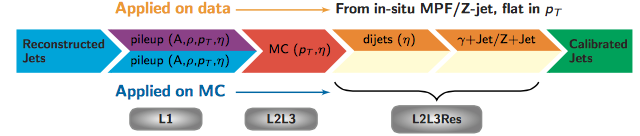
\includegraphics[width=10cm]{images/jecs.png}
\begin{itemize}
\item The minimum correction levels to be applied on any CMS analysis using Monte Carlo and Data are:
\end{itemize}

\begin{block}{Monte Carlo}
L1(Pile Up) + L2(Relative) + L3(Absolute)
\end{block}

\begin{block}{Data}
L1(Pile Up) + L2(Relative) + L3(Absolute) + L2L3 Residuals
\end{block}

\begin{itemize}
\item Any analysis might place higher correction levels if necessary and available. User can check \href{https://twiki.cern.ch/twiki/bin/view/CMS/JECDataMC}{https://twiki.cern.ch/twiki/bin/view/CMS/JECDataMC} to learn about the ``Recommended Jet Energy Corrections and Uncertainties for Data and MC".
\end{itemize}

}
%---------------------------------------------------------------------------------------------------------------------------------------
\subsubsection{JES Uncertainty Sources}
\frame{
\frametitle{JES and Uncertainties}
\begin{block}{Description}
\begin{itemize}
\item The JEC uncertainty sources provide detailed information on JEC uncertainties for use in statistical data analysis. The sources are fully uncorrelated between themselves, but describe JEC variations that are fully correlated within a given source.
\item FIX ME: Should we include how uncertainties are calculated? How they are applied? Sources?
\end{itemize}
\end{block}
}
%---------------------------------------------------------------------------------------------------------------------------------------
\subsection{Collections}
\frame{
	\frametitle{Jet Collections Supported by the JERC Group}
	\begin{itemize}
		\item Clustering algorithms:
		\begin{itemize}
			\item {\color{red}Anti-k$_{T}$}
			\item Cambridge/Aachen - No JEC yet, but might be supported in future if necessary
		\end{itemize}
		\item Cone sizes:
		\begin{itemize}
			\item {\color{red}$R=\{n/10 : 1{\leqslant}n{\leqslant}10\}$}
		\end{itemize}
		\item Jet types:
		\begin{itemize}
			\item {\color{red}PF} - Still in use
			\item {\color{red}PF+CHS} - Default
			\item {\color{red}PF+PUPPI} - Being tested now
			\item PFClusterJet - Coming soon?
			\item {\color{red}Jet Plus Track (JPT)} - Provided by Olga Kodolova
		\end{itemize}
	\end{itemize}
	\textbf{Note}: Items in {\color{red}red} will be available for use in RunII. This amounts to \textbf{32} different payloads.
}
%---------------------------------------------------------------------------------------------------------------------------------------
%---------------------------------------------------------------------------------------------------------------------------------------
\subsection{PUPPI}
%---------------------------------------------------------------------------------------------------------------------------------------


\section{Technical}
\label{sec:technical}
%!TEX root = ../2018_06_13-HATS-LPC-JEC.tex

\subsection{Textfile Format}

\frame{
\frametitle{What form do the corrections come in?}
\framesubtitle{JEC Text Files}
                \begin{figure}
                  \centering
		     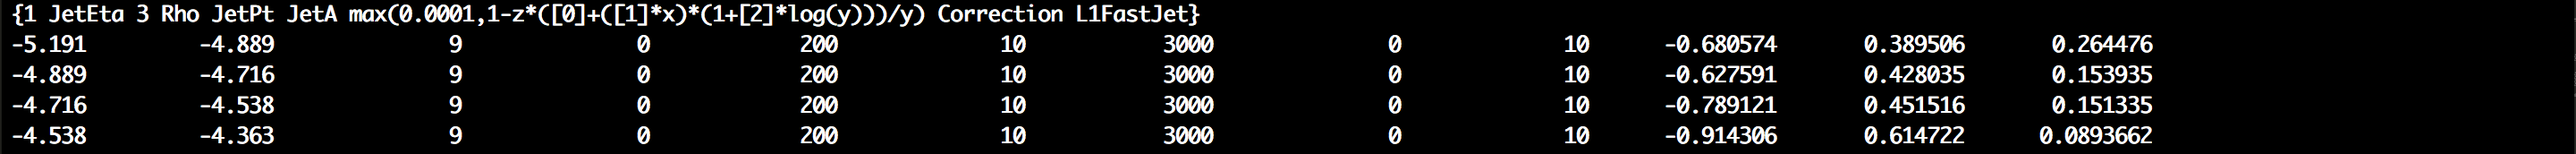
\includegraphics[width=\textwidth]{images/TextFileScreenshots/L1FastJet.png}    
                    \caption{L1FastJet}
                 \end{figure}

                \begin{figure}
                  \centering
		     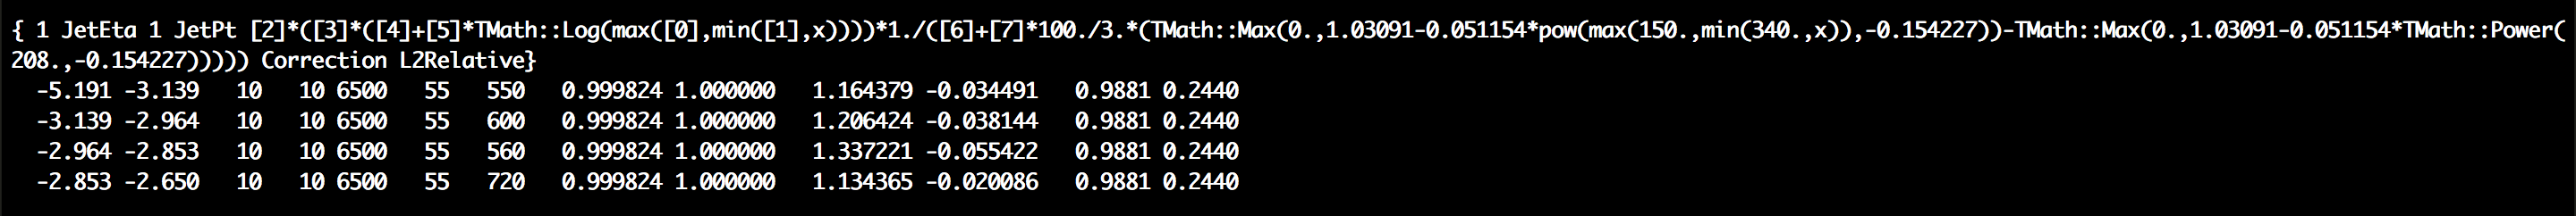
\includegraphics[width=\textwidth]{images/TextFileScreenshots/L2L3Residuals.png}    
                    \caption{L2L3Residuals}
                 \end{figure}

	\vspace{-.5cm}
	\begin{block}{How to read the JEC text files?}
                \begingroup \scriptsize
		\begin{itemize}
		\item The \textbf{top row} establishes the definitions for the parameters to follow, the correction factor and the correction level being applied.
		\item The \textbf{first two columns} are the $\eta$ bin boundaries
		\item The next column tells you how many columns will follow it (in this case 9)
		\item The next numbers define the bin boundaries in e.g. $\rho$, $p_{T}$, and/or jet area
                \item The last numbers are parameters for the correction
		\item Instructions on how to apply the Jet Energy Corrections from a text file in FWLite environment. \\ 
		\href{https://twiki.cern.ch/twiki/bin/view/CMSPublic/WorkBookJetEnergyCorrections}{https://twiki.cern.ch/twiki/bin/view/CMSPublic/WorkBookJetEnergyCorrections}
		\end{itemize}
                \endgroup
	\end{block}
}

\frame{
\frametitle{What form do the corrections come in?}
\framesubtitle{JEC Uncertainty Text Files}
                \begin{figure}
                  \centering
		     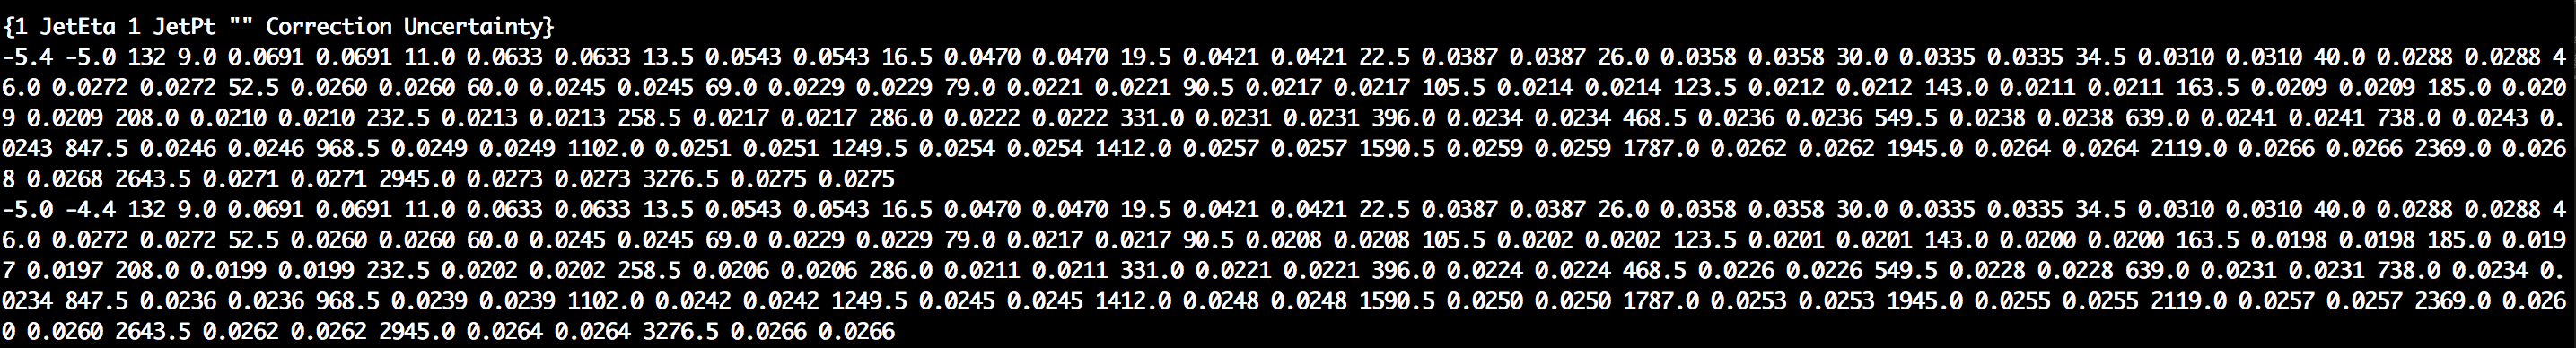
\includegraphics[width=\textwidth]{images/TextFileScreenshots/Uncertainty.png}    
                    \caption{Total Uncertainty}
                 \end{figure}
	\vspace{-.4cm}
                \begin{figure}
                  \centering
	             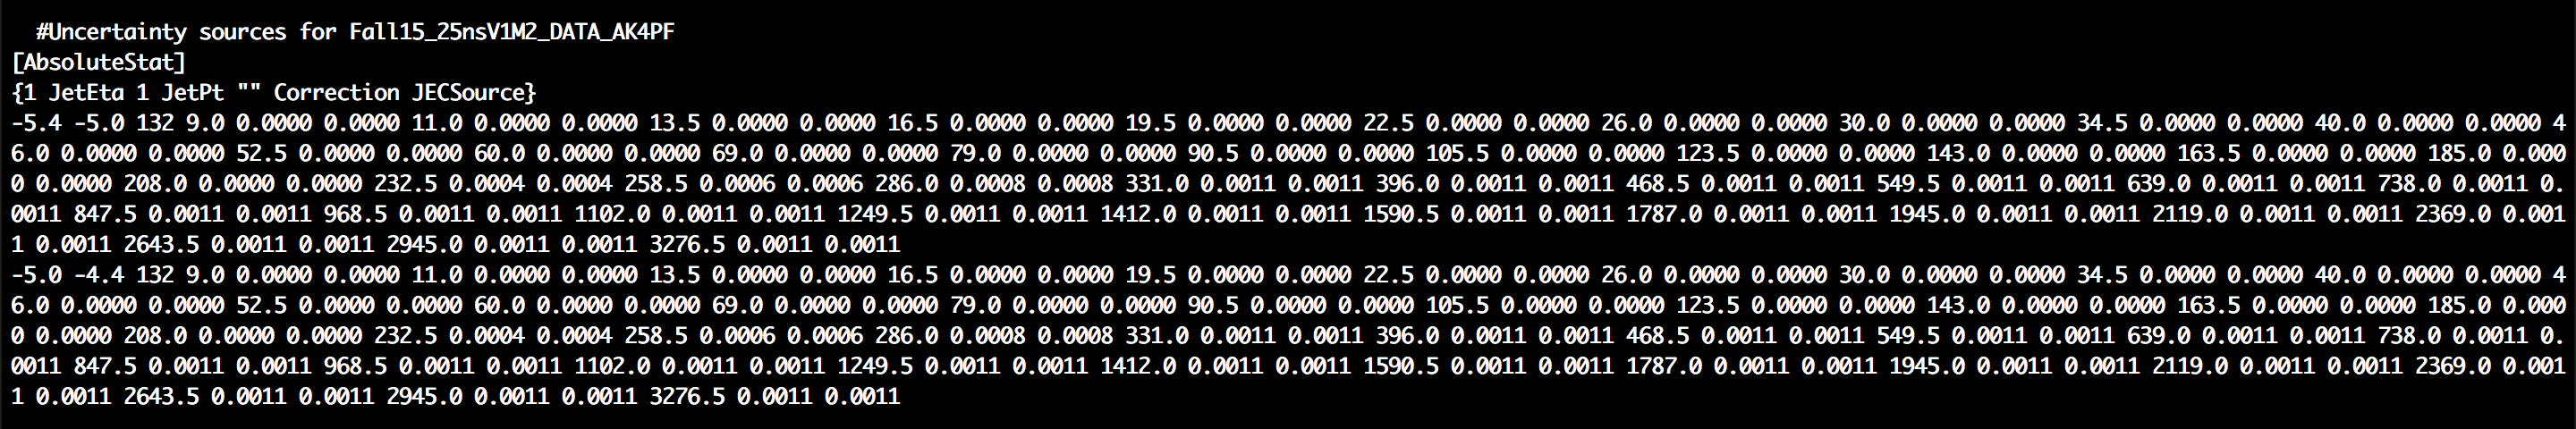
\includegraphics[width=\textwidth]{images/TextFileScreenshots/UncertaintySources.png}    
                    \caption{Uncertainty by Source}
                 \end{figure}

	\vspace{-.5cm}
	\begin{block}{How to read the JEC Uncertainty text files?}
                \begingroup \scriptsize
		\begin{itemize}
                \item First two columns are $\eta$ range, third column is how many columns will follow it
                \item Following this, you have lower $p_T$ bin boundary, uncertainty, upper $p_T$ bin boundary repeated
                \item In file with uncertainties split by source, the name of the source begins each section [LikeThis]
		\end{itemize}
                \endgroup
	\end{block}
}

\frame{
\frametitle{What form do the corrections come in?}
\framesubtitle{JER Text Files}
                \begin{figure}
                  \centering
		     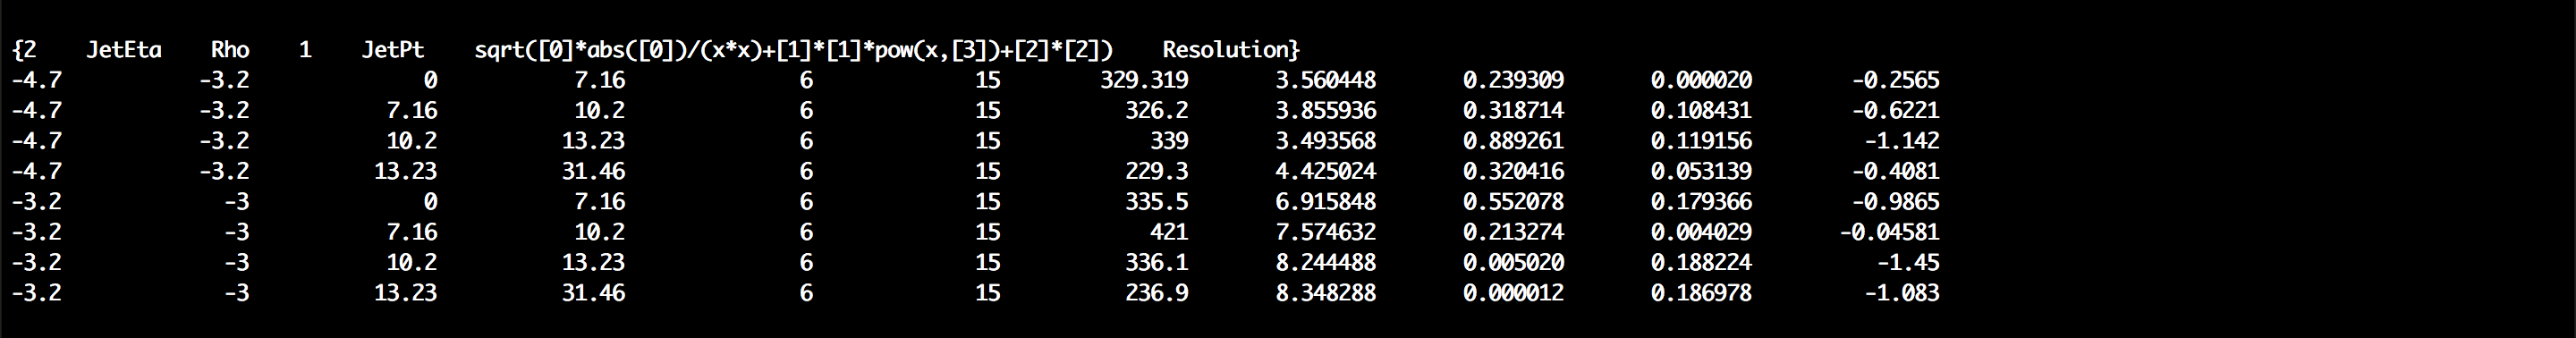
\includegraphics[width=\textwidth]{images/TextFileScreenshots/JetResolutionResolution.png}    
                    \caption{Jet Resolution}
                 \end{figure}
	\vspace{-.4cm}
                \begin{figure}
                  \centering
	             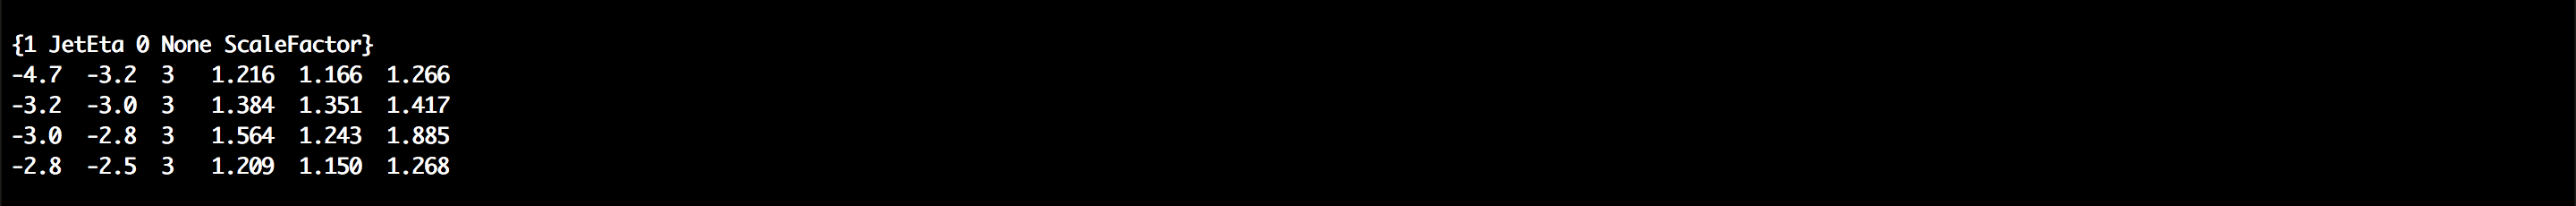
\includegraphics[width=\textwidth]{images/TextFileScreenshots/JetResolutionScaleFactors.png}    
                    \caption{Jet Resolution Scale Facors}
                 \end{figure}

	\vspace{-.5cm}
	\begin{block}{How to read the JER text files?}
                \begingroup \scriptsize
		\begin{itemize}
                \item JER (top): $\eta$ bin boundaries, rho bin boundaries, number of columns to follow, $p_T$ bin boundaries, parameters
                \item JER scale factors (bottom): $\eta$ bin boundaries, number of columns to follow, scale factor, scale factor varied down, scale factor varied up
		\end{itemize}
                \endgroup
	\end{block}
}

%-----------------------------------------------------------------------------------------------------------
\subsection{Textfile Application}
\frame{
\frametitle{What form do the corrections come in?}
\framesubtitle{Global Tag}
\begin{block}{Global Tag}
\begin{itemize}
\item Conditions data are defined in the Offline Conditions Database (ORCOF), which is read in CMSSW applications via Frontier caching servers.
\item The set of dataset tags which together define the offline conditions data are collected together in a \textbf{Global Tag (GT)}, which is itself stored in the database.
\item How to connect to a GT:
\end{itemize} 
\end{block}

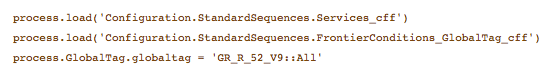
\includegraphics[width=10cm]{images/globaltag.png}

\begin{alertblock}{Note:}
\begin{itemize}
\item There can be many GT's for a given CMSSW release
\item It is important, therefore, that you know which conditions are in the GT you are using
\end{itemize}
\end{alertblock}

}
%-----------------------------------------------------------------------------------------------------------
\frame{
\frametitle{What form do the corrections come in?}
\framesubtitle{How to connect to a local sql file.}
\begin{columns}
\begin{column}{3.5cm}
\begin{block}{}
The recommended way of accessing JEC is with a global tag. The SQLlite file option is mainly used in the initial testing phase in preparation of a global tag.
\end{block}
\end{column}
\begin{column}{8.5cm}
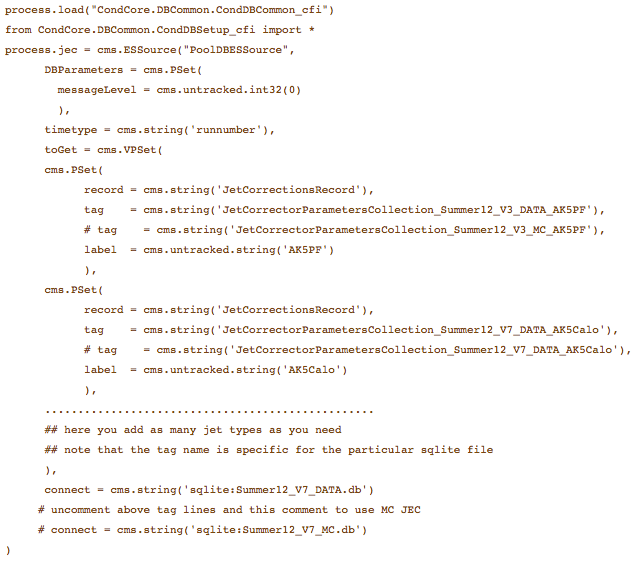
\includegraphics[width=8.5cm]{images/sqlfile.png}
\end{column}
\end{columns}

}
%-----------------------------------------------------------------------------------------------------------
\frame{
\frametitle{What form do the corrections come in?}
\framesubtitle{How to connect to a local sql file.}

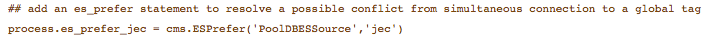
\includegraphics[width=11cm]{images/sql2.png}

\begin{block}{}
\begin{itemize}
\item When using a local SQL file, \textbf{es$\_$prefer} should be added to the process chain in the cfg file.
\item In this case, an \textbf{es$\_$prefer} indicates that whatever is defined in \textbf{es$\_$source} takes precedence over any other source for the condition object (in particular, the global tag).
\end{itemize}
\end{block}

}







\section{User Software}
\label{sec:user_software}
%!TEX root = ../2019_06_04-HATS-LPC-JEC.tex

\subsection{Workflow}
\label{sec:user_software}
%---------------------------------------------------------------------------------------------------------------------------------------
\begin{frame}
	\frametitle{JEC Options - Which path will you take?}
	\begin{textblock}{0.3}(0.72,0.08)
		{\color{RedOrange}\small Not showing NanoAOD!!!}
	\end{textblock}

	\tikzstyle{type} = [ellipse, minimum width=1.5cm, minimum height=1cm, text centered, draw=black, fill=yellow!30, font=\scriptsize]
	\tikzstyle{tier} = [rectangle, rounded corners, minimum width=1.5cm, minimum height=1cm,text centered, draw=black, fill=red!30, font=\scriptsize]
	\tikzstyle{t1}   = [rectangle, rounded corners, minimum width=1.5cm, minimum height=1cm, text centered, draw=black, fill=blue!30, font=\scriptsize]
	\tikzstyle{t2}   = [rectangle, rounded corners, minimum width=1.5cm, minimum height=1cm, text centered, draw=black, fill=orange!30, font=\scriptsize]
	\tikzstyle{t3}   = [rectangle, rounded corners, minimum width=1.5cm, minimum height=1cm, text centered, draw=black, fill=green!30, font=\scriptsize]
	\tikzstyle{arrow}      = [->,>=stealth]
	\tikzstyle{arrowrec}   = [->,>=stealth, thick, violet]
	\tikzstyle{arrownorec} = [->,>=stealth, ultra thick, violet]

	\hspace*{-0.2cm}\begin{tikzpicture}[node distance=2.1cm]
		\node (datatier)[type]                                 {Data Tier};
		\node (jec)     [type, below of=datatier]              {JEC};
		\node (jecu)    [type, below of=jec]                   {JEC Unc.};
		\node (jer)     [type, below of=jecu, text width=1.5cm]{JER\\\tiny(up, nom., down)};

		\node (miniaod) [tier, right of=datatier]           {MINIAOD};
		\node (aod)     [tier, right of=miniaod, xshift=6cm]{AOD};

		\node (default_jec) [t1, right of=jec]                        {MiniAOD};
		\node (tbx)         [t1, right of=default_jec, xshift=-0.45cm]{JetToolbox};
		\node (ajc)         [t1, right of=tbx, xshift=-0.2cm]         {addJetCollection};
		\node (pju)         [t1, right of=ajc, xshift=-0.05cm]        {patJetUpdater};
		\node (pfbreco)     [t1, right of=pju, xshift=-0.35cm]        {PFBRECO};
		\node (otf)         [t1, right of=pfbreco, xshift=-0.5cm]     {on-the-fly};

		\node (prod1) [t2, right of=jecu]                 {Producer};
		\node (otf1)  [t2, right of=prod1, xshift=6cm]{on-the-fly};

		\node (prod2) [t3, right of=jer]                  {Producer};
		\node (otf2)  [t3, right of=prod2, xshift=6cm]{on-the-fly};

		\draw [arrow]      (aod) -- (tbx);
		\draw [arrow]      (aod) -- (ajc);
		\draw [arrow]      (aod) -- (pju);
		\draw [arrow]      (aod) -- (pfbreco);
		\draw [arrow]      (aod) -- (otf);
		\draw [arrow]      (miniaod) -- (default_jec);
		\draw [arrowrec]   (miniaod) -- (tbx);
		\draw [arrow]      (miniaod) -- (ajc);
		\draw [arrownorec] (miniaod) -- (pju);
		\draw [arrow]      (miniaod) -- (pfbreco);
		\draw [arrow]      (miniaod) -- (otf);

		\draw [arrow]      (default_jec) -- (prod1);
		\draw [arrowrec]   (tbx) -- (prod1);
		\draw [arrow]      (ajc) -- (prod1);
		\draw [arrownorec] (pju) -- (prod1);
		\draw [arrow]      (pfbreco) -- (prod1);
		\draw [arrow]      (otf) -- (prod1);
		\draw [arrow]      (default_jec) -- (otf1);
		\draw [arrow]      (tbx) -- (otf1);
		\draw [arrow]      (ajc) -- (otf1);
		\draw [arrow]      (pju) -- (otf1);
		\draw [arrow]      (pfbreco) -- (otf1);
		\draw [arrow]      (otf) -- (otf1);

		\draw [arrownorec] (prod1) -- (prod2);
		\draw [arrow]      (prod1) -- (otf2);
		\draw [arrow]      (otf1) -- (prod2);
		\draw [arrow]      (otf1) -- (otf2);

		\draw[arrownorec] (current bounding box.north) ++(-3em, -0.5em) -- ++(2em, 0) node[right, black, font=\scriptsize] {Favorite (no reclustering)};
		\draw[arrowrec]   (current bounding box.north) ++(-3em, -1.5em) -- ++(2em, 0) node[right, black, font=\scriptsize] {Favorite (with reclustering)};
		\draw[arrow]      (current bounding box.north) ++(-3em, -2.5em) -- ++(2em, 0) node[right, black, font=\scriptsize] {Other option};

	\end{tikzpicture}
\end{frame}


\section{Conclusion}
\label{sec:conclusion}
%!TEX root = ../2019_06_04-HATS-LPC-JEC.tex

\subsection{Conclusion}
\label{sec:conclusion}
%---------------------------------------------------------------------------------------------------------------------------------------
\begin{frame}		
	\frametitle{Conclusion}
	\vspace*{-0.24cm}
	\begin{block}{More sources of information!}
		\begin{itemize}
			\footnotesize
			\item \textbf{JetMET} - Physics Object Group (POG) dedicated to jet and missing transverse momentum performance  -- \href{https://twiki.cern.ch/twiki/bin/view/CMS/JetMET}{Twiki}, \href{https://hypernews.cern.ch/HyperNews/CMS/get/JetMET.html}{Hypernews}, \href{https://indico.cern.ch/category/1308}{Meetings}
			\begin{itemize}
				\footnotesize
				\item Jet Energy Resolutions and Corrections (JERC) Subgroup -- \href{https://twiki.cern.ch/twiki/bin/view/CMS/JetEnergyScale}{Twiki}, \href{https://hypernews.cern.ch/HyperNews/CMS/get/jes.html}{Hypernews}
				\begin{itemize}
					\scriptsize
					\item \href{https://twiki.cern.ch/twiki/bin/view/CMS/JERCReference}{JEC and JER Reference Sample Page}
					\item \href{https://twiki.cern.ch/twiki/bin/view/CMSPublic/WorkBookJetEnergyCorrections?redirectedfrom=CMS.WorkBookJetEnergyCorrections}{WorkBook Page on Jet Energy Corrections}
					\item \href{https://twiki.cern.ch/twiki/bin/view/CMSPublic/WorkBookJetEnergyResolution}{WorkBook Page on Jet Energy Resolution}
					\item SQLite files, text files, and tarballs -- \href{https://github.com/cms-jet/JECDatabase}{JEC Database}, \href{https://github.com/cms-jet/JRDatabase}{JER Database}
				\end{itemize}
				\item JetMET Algorithms and Reconstruction (JMAR) Subgroup -- \href{https://twiki.cern.ch/twiki/bin/view/CMS/JetEnergyScale}{Twiki}, \href{https://hypernews.cern.ch/HyperNews/CMS/get/jet-algorithms.html}{Hypernews}, \href{https://twiki.cern.ch/twiki/bin/view/CMS/JetToolbox}{JetToolbox}
				\item Missing ET (MET) Subgroup -- \href{https://twiki.cern.ch/twiki/bin/view/CMS/MissingET}{Twiki}, \href{https://hypernews.cern.ch/HyperNews/CMS/get/met.html}{Hypernews} 
				\item JetMET DQM and Validation Subgroup -- \href{https://twiki.cern.ch/twiki/bin/view/CMS/JetMETDQMValRun2}{Twiki}, \href{https://hypernews.cern.ch/HyperNews/CMS/get/jetmet-dqm.html}{Hypernews} 
				\item JetMET Trigger -- \href{https://twiki.cern.ch/twiki/bin/viewauth/CMS/JetMETTriggers}{Twiki}, \href{https://hypernews.cern.ch/HyperNews/CMS/get/jetmet-trigger.html}{Hypernews} 
			\end{itemize}
			\item \textbf{FNAL LPC Resources:}
			\begin{itemize}
				\footnotesize
				\item \href{https://indico.cern.ch/category/7082/}{Weekly Run 2 Discussion Groups}
				\item \href{http://lpc.fnal.gov/programs/schools-workshops/hats.shtml}{Hands-On Advanced Tutorial Sessions (HATS)}
			\end{itemize}
			\item MiniAOD Twiki -- \href{https://twiki.cern.ch/twiki/bin/view/CMSPublic/WorkBookMiniAOD2016}{2016}, \href{https://twiki.cern.ch/twiki/bin/view/CMSPublic/WorkBookMiniAOD2017}{2017}
			\item \textbf{Papers:}
			\begin{itemize}
				\footnotesize
				\item JME-13-004 (Run 1) and JME-16-001 (Run 2, in progress)
				\item Particle Flow: PRF-14-001
			\end{itemize}
		\end{itemize}
	\end{block}
\end{frame}


\section{Hands-On}
\label{sec:hands_on}
%!TEX root = ../2015_06_16-HATS-LPC-JEC.tex

\frame{
	\begin{block}{}
		\begin{center}
			\shadowoffset{2pt}
			\shadowcolor{tamugold}
			\shadowtext{{\fontsize{30}{60}\selectfont \textbf{\textcolor{tamumaroon}{Let's look at some code!}}}}
			\vspace{1.5mm}
		\end{center}
	\end{block}
	\centering
	\footnotesize
	\href{https://github.com/cms-jet/JMEDAS}{https://github.com/cms-jet/JMEDAS}\\
	\href{https://github.com/cms-jet/JetMETAnalysis}{https://github.com/cms-jet/JetMETAnalysis}\\
	\href{https://github.com/cms-sw/cmssw/blob/CMSSW_7_5_X/PhysicsTools/PatAlgos/test/update_jets_from_MiniAOD.py}{https://github.com/cms-sw/cmssw/blob/CMSSW\_7\_5\_X/PhysicsTools/PatAlgos/test/update\_jets\_from\_MiniAOD.py}
}
%---------------------------------------------------------------------------------------------------------------------------------------
\fvset{frame=single,framesep=1mm,fontfamily=courier,fontsize=\scriptsize,numbers=left,framerule=.3mm,numbersep=1mm,commandchars=\\\{\}}
\begin{frame}[fragile]
	\frametitle{Setup}
	\framesubtitle{Set environment and check out code}

\begin{Verbatim}[label={Setup Commands}]
# If using TCSH
\textcolor{Orange}{setenv SCRAM_ARCH slc6_amd64_gcc491}
# If site uses cvmfs, like CERN or FNAL
\textcolor{Orange}{source /cvmfs/cms.cern.ch/cmsset_default.csh}
\textcolor{Orange}{source /cvmfs/cms.cern.ch/crab3/crab.csh}
\textcolor{Orange}{cmsrel CMSSW_7_4_2_patch1}
\textcolor{Orange}{cd CMSSW_7_4_2_patch1/src/}
\textcolor{Orange}{cmsenv}
\textcolor{Orange}{git-cms-init}
\end{Verbatim}

\begin{Verbatim}[label={Check out the code for the first exercise}]
\textcolor{Orange}{git cms-addpkg CommonTools/PileupAlgos}
\textcolor{Orange}{git cms-merge-topic nhanvtran:puppi-etadep-741-v1}
\textcolor{Orange}{git clone git@github.com:cms-jet/JetToolbox.git JMEAnalysis/JetToolbox}
	\textcolor{Orange}{ -b jetToolbox_74X}
\textcolor{Orange}{mkdir Analysis}
\textcolor{Orange}{cd Analysis}
\textcolor{Orange}{git clone https://github.com/cms-jet/JMEDAS.git}
\textcolor{Orange}{cd ..}
\textcolor{Orange}{scram b -j 8}
\textcolor{Orange}{cd Analysis/JMEDAS/test}
\textcolor{Orange}{voms-proxy-init -voms cms --valid 192:00}
\end{Verbatim}

\end{frame}

\begin{frame}[fragile]
	\frametitle{Setup}
	\framesubtitle{Set environment and check out code}

\begin{Verbatim}[label={Setup Commands}]
# If using TCSH
\textcolor{Orange}{setenv SCRAM_ARCH slc6_amd64_gcc491}
# If site uses cvmfs, like CERN or FNAL
\textcolor{Orange}{source /cvmfs/cms.cern.ch/cmsset_default.csh}
\textcolor{Orange}{source /cvmfs/cms.cern.ch/crab3/crab.csh}
\textcolor{Orange}{cmsrel CMSSW_7_4_2_patch1}
\textcolor{Orange}{cd CMSSW_7_4_2_patch1/src/}
\textcolor{Orange}{cmsenv}
\textcolor{Orange}{git-cms-init}
\end{Verbatim}

\begin{Verbatim}[label={Check out the code for the first exercise}]
\textcolor{Orange}{git cms-addpkg CommonTools/PileupAlgos}
\textcolor{Orange}{git cms-merge-topic nhanvtran:puppi-etadep-741-v1}
\textcolor{Orange}{git clone git@github.com:cms-jet/JetToolbox.git JMEAnalysis/JetToolbox}
	\textcolor{Orange}{ -b jetToolbox_74X}
\textcolor{Orange}{mkdir Analysis}
\textcolor{Orange}{cd Analysis}
\textcolor{Orange}{git clone https://github.com/cms-jet/JMEDAS.git}
\textcolor{Orange}{cd ..}
\textcolor{Orange}{scram b -j 8}
\textcolor{Orange}{cd Analysis/JMEDAS/test}
\textcolor{Orange}{voms-proxy-init -voms cms --valid 192:00}
\end{Verbatim}

	\begin{textblock}{12.3}(0.25,4.0)
		\begin{figure}
			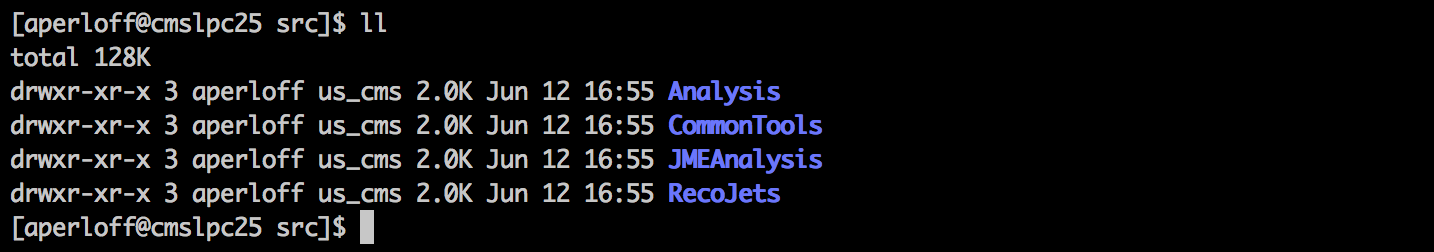
\includegraphics[width=\textwidth]{images/setup_software}
			\label{fig:setup_software}
		\end{figure}
	\end{textblock}

\end{frame}

%---------------------------------------------------------------------------------------------------------------------------------------
\begin{frame}[fragile]
	\frametitle{Exercise 1}
	\framesubtitle{pat::jets}

\begin{Verbatim}[label={Exercise 1}]
# Run with AODSIM + jetToolbox
# Run with MiniAODSIM + jetToolbox
# Run with MiniAODSIM + PAT
# In all of these cases you don't need to worry about double correcting
#     because you're reclustering jets and don't already have any corrections
\textcolor{Orange}{cmsRun jmehats_JEC.py}
\end{Verbatim}

\begin{block}{}
	\begin{itemize}
		\item Try playing around with the \textbf{doMiniAOD} and \textbf{doJetToolbox} options
		\item Change the jet collections and the correction levels
		\item \textbf{Hint}: For no corrections it seems you need to include just the L3Absolute corrections
		\item Explor the trees you make with this program
		\item If you have AK4PF and AK4PFchs in your tree you can use the plots\_jec\_hats\_1.py to make some distributions
	\end{itemize}
\end{block}

\end{frame}

%---------------------------------------------------------------------------------------------------------------------------------------
\begin{frame}[fragile]
	\frametitle{Exercise 2}
	\framesubtitle{Uncorrect and recorrect jets from MiniAOD}

\begin{Verbatim}[label={Exercise 2}]
# You need to worry about double correcting if you are grabbing jets
#     from MiniAODSIM file directly
\textcolor{Orange}{git-cms-addPkg PhysicsTools/PatAlgos}
\textcolor{Orange}{cd PhysicsTools/PatAlgos/test/}
\textcolor{Orange}{cmsRun update_jets_from_MiniAOD.py}
\end{Verbatim}

\begin{block}{}
	\begin{itemize}
		\item Take a look at \href{https://github.com/cms-sw/cmssw/pull/8288}{https://github.com/cms-sw/cmssw/pull/8288}
		\item Explor the output of the program
	\end{itemize}
\end{block}

\end{frame}

%---------------------------------------------------------------------------------------------------------------------------------------
\begin{frame}[fragile]
	\frametitle{Exercise 3}
	\framesubtitle{Jet corrections on-the-fly}

\begin{Verbatim}[label={Exercise 3}]
\textcolor{Orange}{cmsRun Analysis/JMEDAS/test/jmedas_fwlite.py}
\end{Verbatim}

\begin{block}{}
	\begin{itemize}
		\item Take a look at the code and identify the lines which specify the JEC
		\item If you run over the same file and with the same set of JEC do your jets end up being the same?
	\end{itemize}
\end{block}

\end{frame}

%---------------------------------------------------------------------------------------------------------------------------------------
\begin{frame}[fragile]
	\frametitle{Exercise 4}
	\framesubtitle{reco::jets (AODSIM $+$ PFBRECO)}

\begin{Verbatim}[label={Exercise 4}]
# Run with AODSIM + PFBRECO
# not much worry about double correcting because AODSIM jets, or reclustered jets,
#     beacuse you do not have corrections already applied
\textcolor{Orange}{cd CMSSW_7_4_2_patch1/src/}
\textcolor{Orange}{git clone git@github.com:cms-jet/JetMETAnalysis.git}
\textcolor{Orange}{scram b -j 8}
\textcolor{Orange}{cd JetMETAnalysis/JetAnalyzers/test/}
\textcolor{Orange}{cmsRun run_JRA_cfg.py}
\end{Verbatim}

\begin{block}{}
	\begin{itemize}
		\item This is the same code we have been using to make the MC-truth corrections
		\item We will be moving to the JMEValidator code, which uses the JetToolbox
		\item This is a good example of both PFBRECO
		\item You can also look at bin/jet\_correction\_analyzer\_x.cc if you need another example of correcting jets on-the-fly
		\item Code located at \href{https://github.com/cms-jet/JetMETAnalysis}{https://github.com/cms-jet/JetMETAnalysis}
	\end{itemize}
\end{block}

\end{frame}

%---------------------------------------------------------------------------------------------------------------------------------------
\begin{frame}[fragile]
	\frametitle{Exercise 5}
	\framesubtitle{Jet Energy Resolution (JER) \& Uncertainties}

\begin{Verbatim}[label={Exercise 5}]
# Go back to jmehats_JEC.py and turn on either JER, uncertainties, or both
# JER also has the option to scale 1 sigma up or down from the nominal values
\textcolor{Orange}{cmsRun jmedas_JEC.py}
\end{Verbatim}

\begin{block}{}
	\begin{itemize}
		\item The JER factors are taken from \href{https://twiki.cern.ch/twiki/bin/view/CMS/JetResolution#JER_Scaling_factors_and_Uncertai}{https://twiki.cern.ch/twiki/bin/view/CMS/JetResolution\#JER\_Scaling\_factors\_and\_Uncertai}
		\item Because we have no data these have not been updated with $13\unit{TeV}$ resolution factors
	\end{itemize}
\end{block}

\end{frame}





\section*{Backup}
\label{sec:backup}
%!TEX root = ../2015_06_16-HATS-LPC-JEC.tex

\frame{
	\begin{block}{}
		\begin{center}
			\shadowoffset{2pt}
			\shadowcolor{tamugold}
			\shadowtext{{\fontsize{30}{60}\selectfont \textbf{\textcolor{tamumaroon}{Backup Slides}}}}
			\vspace{1.5mm}
		\end{center}
	\end{block}
}
%---------------------------------------------------------------------------------------------------------------------------------------
\begin{comment}
\subsection{How do we guarantee we are correcting what we think we are correcting?}
\frame{
	\frametitle{How do we guarantee we are correcting what we think we are correcting?}

	Pileup - match same jet without PU to jet with PU. Litterally the only difference is the additional energy due to PU. Can't be anything else...maybe small matching uncertainty

	L2L3 MCTruth - We in in jet pt as well as ref pt and eta so that we are independent of the jet pt spectrum. Otherwise our corrections would only be valid for sampels with the same pt spectrum (because the average energies would be different)
	
	L5 - second order correction to L2L3, but binned in flavor. Same type of correction though (response based). Again, binned in jet pt, ref pt, and eta.
	
	L2L3Res - make sure that we are measuring the dijet case by using an $\alpha<0.3$ cut. Then we extrapolate to the $\alpha=0$ value. This means that the pt of any third jet is really low. Then take the ratio of MC/data. Thus we are really measuring the difference of MC to data in the dijet case.
}
\end{comment}

\end{document}
